\documentclass[aspectratio=169,11pt]{beamer}

\usepackage[T1]{fontenc}
\usepackage[utf8]{inputenc}
\usepackage{amsmath,amssymb,bm}
\usepackage{booktabs}
\usepackage{graphicx}
\usepackage{listings}
\usepackage{xcolor}

% -----------------------------------------------------------------------------
% A deliberately simple visual system. The deck is being used as a structured
% draft of the paper, so typography, equations, tables, and figures carry the
% hierarchy rather than decorative slide elements.
% -----------------------------------------------------------------------------
\definecolor{Accent}{HTML}{6E4E8E}
\definecolor{AccentLight}{HTML}{F4F1F7}
\definecolor{Ink}{HTML}{151515}
\definecolor{Body}{HTML}{444444}
\definecolor{Muted}{HTML}{737373}
\definecolor{MapBlue}{HTML}{0072BD}
\definecolor{Co2Orange}{HTML}{D95319}

\usetheme{default}
\setbeamertemplate{navigation symbols}{}
\setbeamertemplate{headline}{}
\setbeamertemplate{footline}{%
  \hfill\raisebox{0.25cm}{\color{Muted}\scriptsize\insertframenumber}\hspace{0.45cm}}
\setbeamertemplate{itemize items}[circle]
\setbeamercolor{normal text}{fg=Body,bg=white}
\setbeamercolor{frametitle}{fg=Ink,bg=white}
\setbeamercolor{title}{fg=Ink}
\setbeamercolor{subtitle}{fg=Body}
\setbeamercolor{structure}{fg=Accent}
\setbeamerfont{normal text}{size=\fontsize{12.7}{16.3}\selectfont}
\setbeamerfont{frametitle}{size=\fontsize{20.5}{23}\selectfont,series=\mdseries}
\setbeamerfont{title}{size=\fontsize{24.5}{28}\selectfont,series=\mdseries}
\setbeamerfont{subtitle}{size=\fontsize{14.5}{18}\selectfont}
\setbeamersize{text margin left=0.70cm,text margin right=0.70cm}

\newcommand{\PETCOtwo}{P_{\mathrm{ET}}CO_2}
\newcommand{\MAP}{\mathrm{MAP}}
\newcommand{\CBFV}{\mathrm{CBFV}}
\newcommand{\Amodel}{A_{\mathrm{model}}}
\newcommand{\sectionlabel}[1]{%
  {\color{Accent}\fontsize{8}{9.5}\selectfont\bfseries\MakeUppercase{#1}}\par\vspace{0.12cm}}
\newcommand{\sourcefooter}[1]{%
  \par\vfill{\color{Muted}\fontsize{6.8}{8}\selectfont #1}}
\newcommand{\proofnote}{%
  \sourcefooter{Evidence status: \texttt{proof250}, 250-family presentation proof of concept; not final-paper evidence.}}

\newenvironment{equationcallout}
  {\begin{beamercolorbox}[rounded=true,sep=0.28cm,center,wd=0.94\textwidth]{block body}%
   \setbeamercolor{block body}{bg=AccentLight,fg=Ink}\large}
  {\end{beamercolorbox}}

\newcommand{\sectionframe}[3]{%
  \begin{frame}[plain]
    \vspace{0.7cm}
    {\color{Accent}\fontsize{10}{12}\selectfont\bfseries SECTION #1}\par\vspace{0.45cm}
    {\color{Ink}\fontsize{24.5}{28}\selectfont #2}\par\vspace{0.55cm}
    {\color{Body}\fontsize{14.5}{19}\selectfont #3}
  \end{frame}}

\lstdefinestyle{matlabslide}{
  language=Matlab,
  basicstyle=\ttfamily\fontsize{8.8}{10.8}\selectfont,
  keywordstyle=\color{Accent}\bfseries,
  commentstyle=\color{Muted},
  stringstyle=\color{Co2Orange},
  frame=single,
  rulecolor=\color{Accent!35},
  backgroundcolor=\color{AccentLight!55},
  columns=fullflexible,
  keepspaces=true,
  showstringspaces=false,
  breaklines=true
}

\title{Evaluating Two-Input Transfer Function Analysis of Cerebral Hemodynamics}
\subtitle{Known-truth simulation framework and a 250-family proof of concept}
\author{Amogh Naganand}
\date{August 2026}

\begin{document}

% =============================================================================
% Title and purpose
% =============================================================================

\begin{frame}[plain]
  \titlepage
  \vspace{-0.35cm}
  \begin{center}
    {\color{Accent}\rule{0.28\textwidth}{0.8pt}}
  \end{center}
\end{frame}

\begin{frame}{How this presentation is being used}
\sectionlabel{Purpose}
This presentation is organized like a developing paper rather than a short
conference talk. The early sections establish the signal-processing and
physiological reasoning step by step. The later sections define the simulation,
show how estimates are compared with known truth, and then introduce the first
proof-of-concept results.

\vspace{0.45cm}
The goal is not to make the two-input model look better by default. The goal is
to identify the conditions in which jointly estimating MAP and $\PETCOtwo$
recovers their separate contributions to CBFV more accurately than treating each
input alone.
\end{frame}

% =============================================================================
% Section 1
% =============================================================================

\section{Introduction and motivation}
\sectionframe{1}{Introduction and Motivation}{%
CBFV is influenced by more than arterial pressure. That creates a reason to
consider two inputs, but it does not guarantee that a larger model will be more
accurate.}

\begin{frame}{Cerebral blood flow is regulated despite changing pressure}
\sectionlabel{Introduction and Motivation}
The brain requires continuous blood flow even though systemic arterial pressure
changes from moment to moment. Cerebral autoregulation describes part of the
vascular response that limits how strongly these pressure fluctuations alter
cerebral perfusion. Dynamic cerebral autoregulation focuses on changes occurring
over seconds to minutes and is commonly studied by treating MAP as an input and
CBFV as an output.

\vspace{0.4cm}
Transfer function analysis is useful because it describes this relationship at
each frequency. Gain represents the size of the response and phase represents its
timing. These measures describe a dynamic relationship; they do not prove that
one signal is the only physiological cause of the other.
\sourcefooter{Methodological basis: Zhang et al. (1998), doi:10.1152/ajpheart.1998.274.1.H233; Claassen et al. (2016), doi:10.1177/0271678X15626425; Panerai et al. (2023), doi:10.1177/0271678X221119760.}
\end{frame}

\begin{frame}{$\PETCOtwo$ creates a second measured influence on CBFV}
\sectionlabel{Introduction and Motivation}
Carbon dioxide changes cerebrovascular tone and can influence CBFV in frequency
ranges that overlap with the ranges used for autoregulation analysis. End-tidal
carbon dioxide is not identical to arterial carbon dioxide, but it provides a
continuous practical measurement during resting recordings.

\vspace{0.4cm}
If MAP and $\PETCOtwo$ share fluctuations, a MAP-only transfer function can
contain variation associated with both pathways. The same issue can occur in the
reverse direction for a $\PETCOtwo$-only estimate. Separate SISO estimates remain
valid pairwise descriptions, but they should not automatically be interpreted as
fully separated physiological pathways.
\sourcefooter{$CO_2$ influence and multivariable motivation: Panerai et al. (1999), doi:10.1088/0967-3334/20/3/304; Panerai et al. (2000), doi:10.1109/10.827312; Peng et al. (2008), doi:10.1007/s10439-007-9412-9.}
\end{frame}

\begin{frame}{The study asks a conditional question}
\sectionlabel{Introduction and Motivation}
A two-input model provides a mathematical way to separate shared information,
but it must estimate two pathway coefficients from the same finite recording.
When the inputs are difficult to distinguish, the joint spectral system can
become sensitive to small estimation errors.

\vspace{0.45cm}
The useful question is therefore: \emph{under which combinations of input
relationship, pathway strength, recording quality, and estimator settings does
MISO recover the known pathways more accurately than separate SISO models?}
Human recordings cannot answer this accuracy question by themselves because the
true physiological transfer functions are not directly observable.
\end{frame}

\begin{frame}{SISO and MISO answer related but different questions}
\sectionlabel{Introduction and Motivation}
\begin{center}
  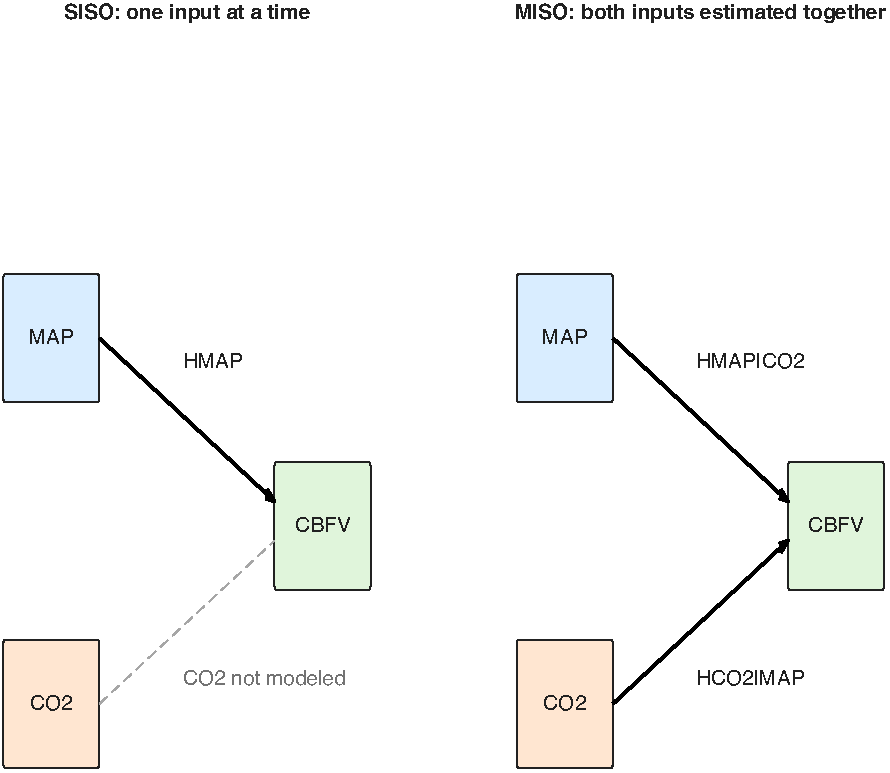
\includegraphics[height=0.68\textheight]{figures/proof250/G01_P01_siso_miso_concept.pdf}
\end{center}
\sourcefooter{Conceptual method diagram generated by the MATLAB project; it does not present numerical evidence.}
\end{frame}

% =============================================================================
% Section 2
% =============================================================================

\section{From time signals to spectra}
\sectionframe{2}{From Physiological Signals to Spectral Estimates}{%
Transfer functions are estimated from auto-spectra and cross-spectra. The
foundation begins with how a finite time signal becomes a stable spectral
estimate.}

\begin{frame}{A transfer function maps an input to an output}
\sectionlabel{Signal-Processing Background}
If $x(t)$ is an input and $y(t)$ is an output, a simple static analogy is
$y=mx$: the slope $m$ describes how strongly the input is represented in the
output. A transfer function plays a similar role but can have a different value
at every frequency and can also describe timing.

\vspace{0.40cm}
\begin{equationcallout}
\[
Y(f)=H(f)X(f)
\]
\end{equationcallout}

\vspace{0.30cm}
The magnitude $|H(f)|$ is gain, while the angle $\angle H(f)$ is phase. Together
they describe the size and timing of the output response at frequency $f$.
\end{frame}

\begin{frame}{The frequency domain reorganizes the same signal}
\sectionlabel{Signal-Processing Background}
MAP, $\PETCOtwo$, and CBFV are first recorded in the time domain. Each sample
describes the signal at one time, which is useful for seeing trends, artifacts,
noise, and timing relationships. Several oscillations can overlap in a single
time trace, however, making their individual contributions hard to see.

\vspace{0.45cm}
The Fourier transform reorganizes that finite record into discrete frequency
values. Slow oscillations appear at low frequencies and faster oscillations at
higher frequencies. Each Fourier value is generally complex: its magnitude
describes the strength of that component and its angle describes phase relative
to a reference sinusoid.
\end{frame}

\begin{frame}{The Fourier transform exposes the frequencies inside the signal}
\sectionlabel{Signal-Processing Background}
\begin{center}
  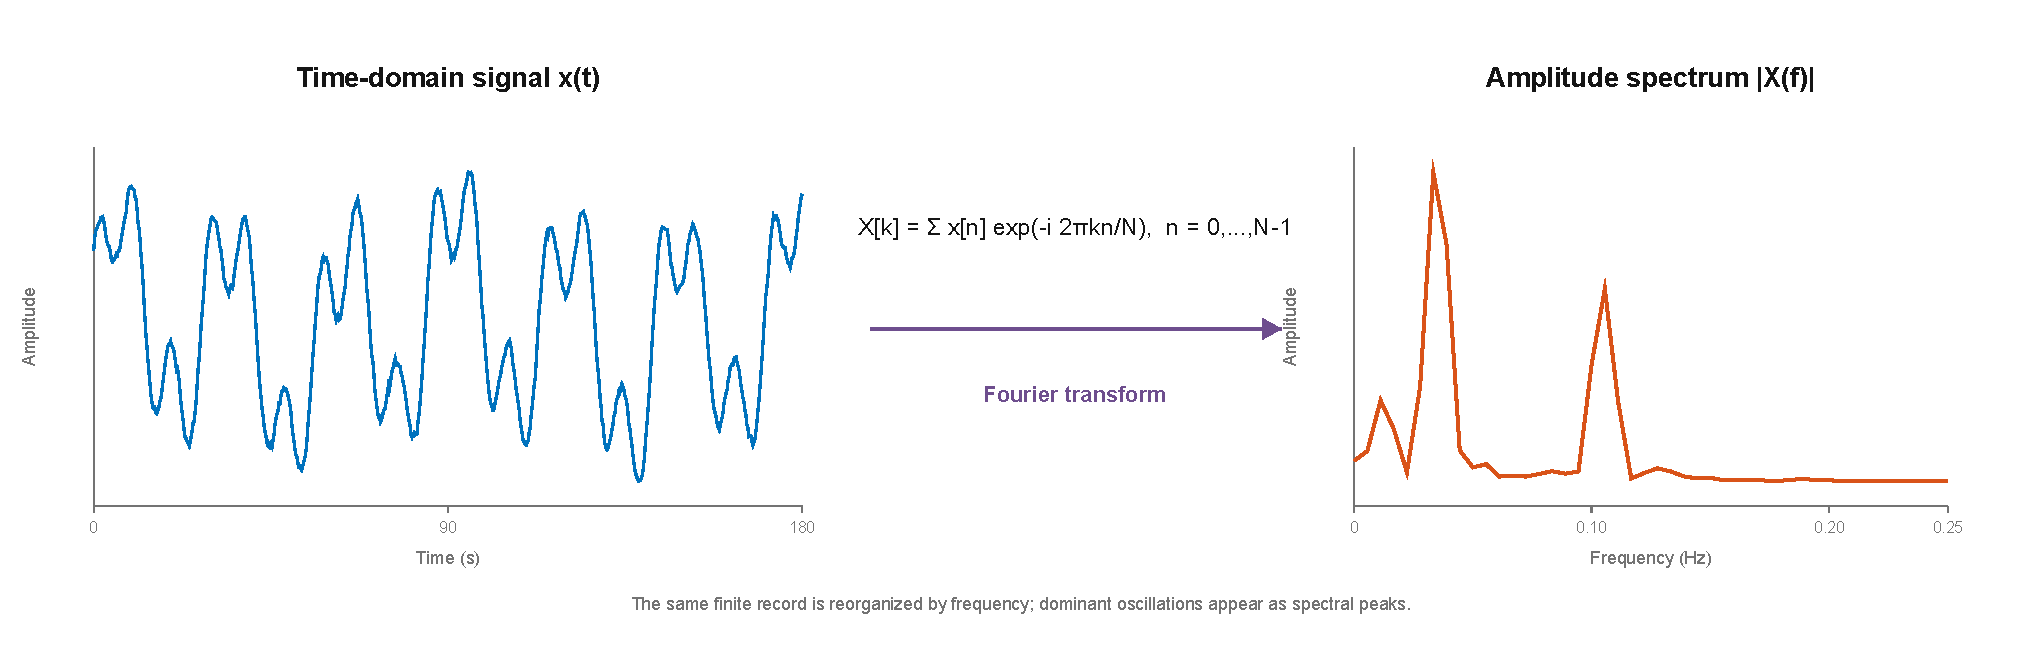
\includegraphics[width=0.96\textwidth]{figures/methods/fourier_transform_visual.pdf}
\end{center}
\sourcefooter{Generated from a sampled signal by \texttt{figure\_generators/generate\_method\_figures.py}; the peaks correspond to oscillations present in the time trace.}
\end{frame}

\begin{frame}{A complex spectrum stores both amplitude and phase}
\sectionlabel{Signal-Processing Background}
Every Fourier value can be written in polar form. Its magnitude gives the
strength of that frequency component, while its angle gives the component's
phase relative to the time origin.

\vspace{0.30cm}
\begin{equationcallout}
\[
X(f)=|X(f)|e^{i\angle X(f)}.
\]
\end{equationcallout}

\vspace{0.20cm}
A power spectrum is based on $|X(f)|^2$ and is therefore real and nonnegative.
It describes how the signal's power is distributed across frequency, but it no
longer retains the phase of the original Fourier value. A cross-spectrum uses
two signals and remains complex, so it can retain their relative phase.
\end{frame}

\begin{frame}{Welch's method creates repeated estimates inside one record}
\sectionlabel{Signal-Processing Background}
Welch's method divides the original record into shorter, often overlapping
segments. Every segment contains the actual samples from its corresponding time
interval; overlapping segments share some of those samples rather than creating
different versions of the signal.

\vspace{0.4cm}
Each segment is multiplied by a window such as a Hann window, transformed, and
converted into a segment-level spectral estimate. Because all segments use the
same frequency grid, their periodograms or cross-periodograms can be averaged
frequency by frequency. This reduces variance but creates a tradeoff: shorter
windows provide more averages, whereas longer windows provide finer frequency
resolution.
\sourcefooter{Spectral-estimation basis: Welch (1967), doi:10.1109/TAU.1967.1161901; current cerebral-TFA recommendations: Panerai et al. (2023), doi:10.1177/0271678X221119760.}
\end{frame}

\begin{frame}{Two routes from one time signal to a spectral estimate}
\sectionlabel{Signal-Processing Background}
\begin{center}
  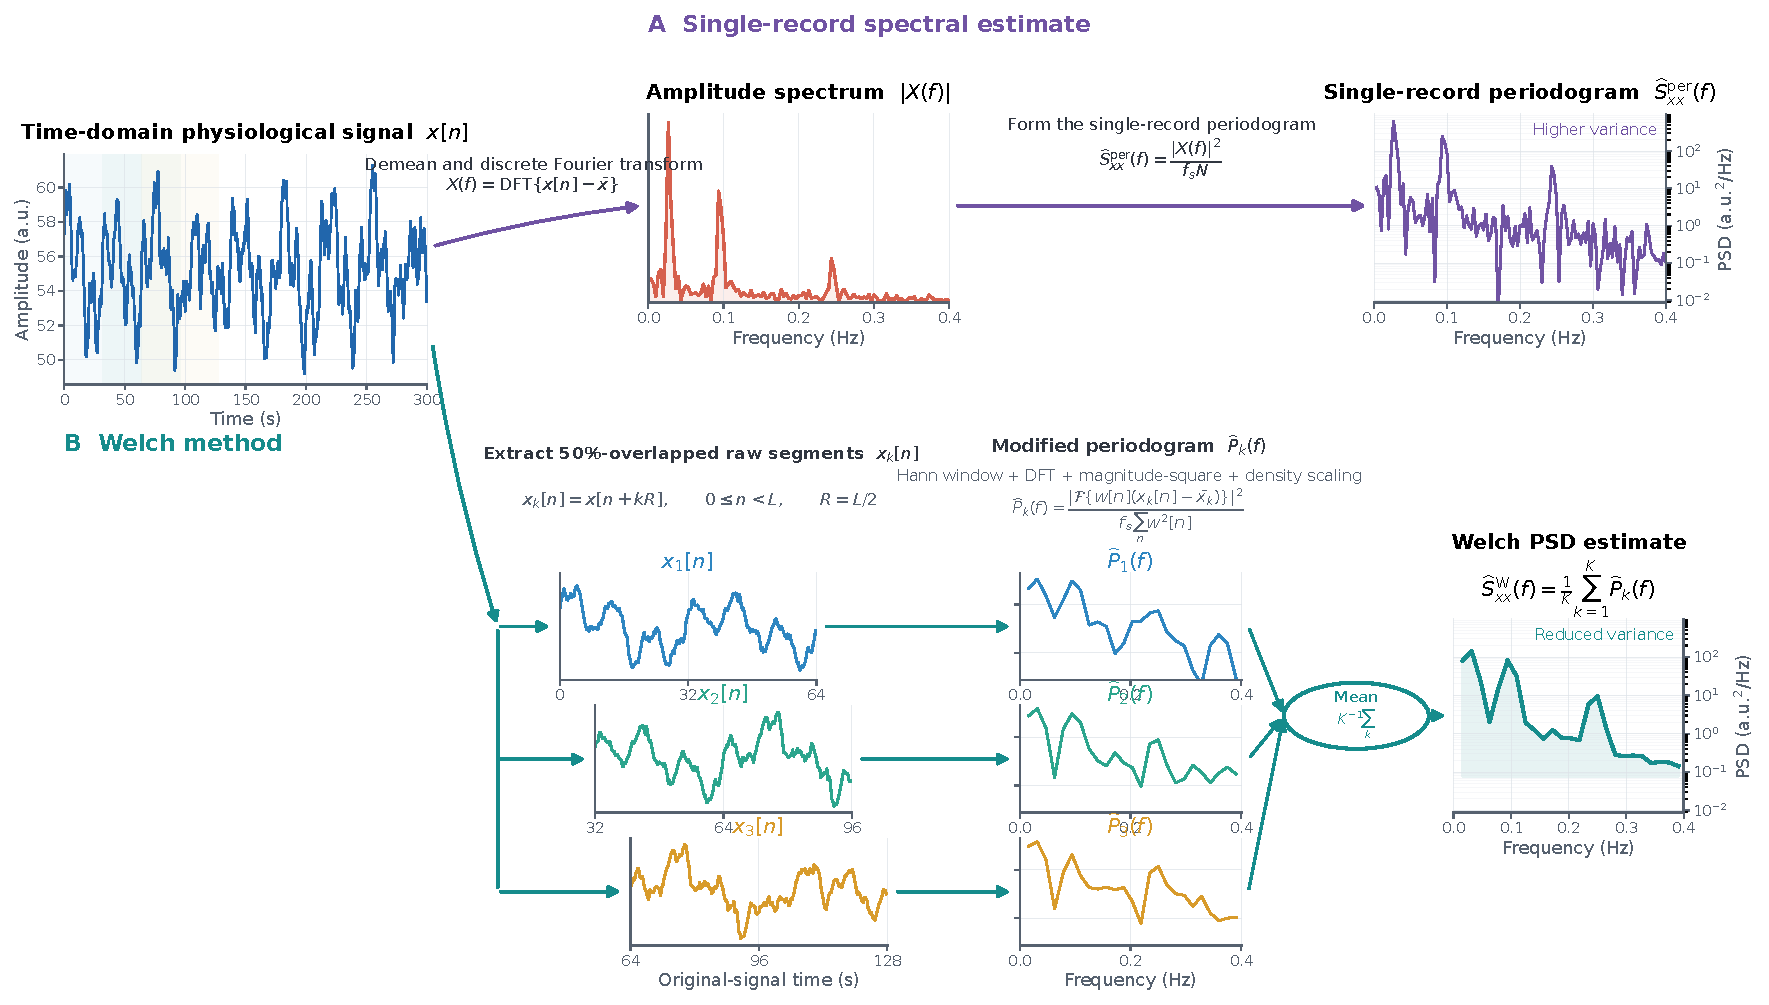
\includegraphics[height=0.63\textheight]{figures/methods/spectral_estimation_routes.pdf}
\end{center}
\sourcefooter{The lower route shows overlapping samples from one signal, segment-level modified periodograms, and their frequency-by-frequency average.}
\end{frame}

\begin{frame}{Auto-spectra describe power within one signal}
\sectionlabel{Signal-Processing Background}
For segment $m$, let $X_m(f)$ be the Fourier transform of the windowed signal.
The segment power estimate contains the product of the complex value and its own
complex conjugate. Welch's estimate averages these products across the $M$
available segments.

\vspace{0.35cm}
\begin{equationcallout}
\[
\widehat S_{xx}(f)
=\frac{1}{M}\sum_{m=1}^{M}X_m^*(f)X_m(f)
=\frac{1}{M}\sum_{m=1}^{M}|X_m(f)|^2
\]
\end{equationcallout}

\vspace{0.25cm}
The implementation also includes the sampling-frequency and window-energy
normalization needed for a correctly scaled power spectral density.
\end{frame}

\begin{frame}{Cross-spectra retain the relationship between two signals}
\sectionlabel{Signal-Processing Background}
For an input $X$ and output $V$, the cross-spectrum uses the conjugate of the
first signal and the Fourier value of the second signal. Its magnitude describes
shared frequency content, while its angle contains the relative phase.

\vspace{0.35cm}
\begin{equationcallout}
\[
\widehat S_{xV}(f)
=\frac{1}{M}\sum_{m=1}^{M}X_m^*(f)V_m(f)
\]
\end{equationcallout}

\vspace{0.25cm}
The ordering must be stated because reversing the two signals conjugates the
cross-spectrum and changes the sign of phase.
\end{frame}

\begin{frame}[fragile]{The code implementation follows the spectral definitions}
\sectionlabel{Code Implementation}
\begin{lstlisting}[style=matlabslide]
Sxx = 0;
SxV = 0;
for m = 1:M
    X = fft(window .* xSegment(:,m));
    V = fft(window .* vSegment(:,m));
    Sxx = Sxx + conj(X).*X;
    SxV = SxV + conj(X).*V;
end
Sxx = Sxx/M;
SxV = SxV/M;
\end{lstlisting}
\sourcefooter{Conceptual implementation. Production functions additionally apply PSD normalization, smoothing, and input checks.}
\end{frame}

% =============================================================================
% Section 3
% =============================================================================

\section{Conventional SISO TFA}
\sectionframe{3}{Conventional SISO Transfer-Function Analysis}{%
The SISO estimator describes one selected input-output relationship at a time.}

\begin{frame}{A dynamic time-domain response becomes multiplication by frequency}
\sectionlabel{SISO Transfer-Function Analysis}
Let $x(t)$ be one selected input and let $v(t)$ be CBFV. The output at one time
can depend on the current and previous values of the input. The impulse response
$h(t)$ describes those delayed and distributed effects, while $e(t)$ contains
output variation not explained by this SISO model.

\vspace{0.30cm}
\begin{align*}
v(t)&=(h*x)(t)+e(t),\\[0.15cm]
V(f)&=H(f)X(f)+E(f).
\end{align*}

The Fourier transform changes convolution into a frequency-by-frequency
multiplication. This is why transfer function analysis can estimate the dynamic
relationship separately at each frequency.
\end{frame}

\begin{frame}{Direct FFT division makes the unexplained term visible}
\sectionlabel{SISO Transfer-Function Analysis}
Dividing the frequency-domain equation by $X(f)$ gives useful intuition, but it
does not isolate the true pathway when the finite record contains unexplained
output variation.

\vspace{0.30cm}
\begin{equationcallout}
\[
\frac{V(f)}{X(f)}
=H(f)+\frac{E(f)}{X(f)}.
\]
\end{equationcallout}

\vspace{0.25cm}
If $X(f)$ is small, even modest unexplained variation can dominate the ratio.
A single FFT ratio also depends heavily on the particular finite realization.
The estimator therefore creates products that can be averaged across Welch
segments rather than dividing two individual Fourier values.
\end{frame}

\begin{frame}{Multiplying by the input conjugate creates spectral products}
\sectionlabel{SISO Transfer-Function Analysis}
Multiply both sides of $V(f)=H(f)X(f)+E(f)$ by the complex conjugate of the
input. The pathway is now multiplied by input power rather than appearing below
an individual Fourier value.

\vspace{0.30cm}
\begin{equationcallout}
\[
X^*(f)V(f)
=H(f)X^*(f)X(f)+X^*(f)E(f).
\]
\end{equationcallout}

\vspace{0.25cm}
The first product becomes the input-output cross-spectrum after averaging. The
second product becomes the input auto-spectrum. The remaining product describes
any systematic relationship between the input and the unexplained output term.
\end{frame}

\begin{frame}{Averaging isolates the modeled relationship in expectation}
\sectionlabel{SISO Transfer-Function Analysis}
Taking the expectation, which Welch averaging approximates using finite
segments, gives

\vspace{0.22cm}
\[
\mathbb E[X^*V]
=H(f)\mathbb E[X^*X]+\mathbb E[X^*E].
\]

If the unexplained output term is not systematically related to the input, then
$\mathbb E[X^*E]\approx0$. The remaining terms are the cross-spectrum and
auto-spectrum:

\vspace{0.18cm}
\begin{equationcallout}
\[
S_{xV}(f)=H(f)S_{xx}(f).
\]
\end{equationcallout}
\end{frame}

\begin{frame}{The SISO estimator follows by solving the spectral equation}
\sectionlabel{SISO Transfer-Function Analysis}
Solving $S_{xV}=HS_{xx}$ for the pathway gives the familiar estimator. Hats
indicate spectra and transfer functions estimated from a finite observation.

\vspace{0.28cm}
\begin{equationcallout}
\[
\widehat H_{x}^{\mathrm{SISO}}(f)
=\frac{\widehat S_{xV}(f)}{\widehat S_{xx}(f)},
\qquad
\widehat G(f)=|\widehat H(f)|,
\qquad
\widehat\phi(f)=\angle\widehat H(f).
\]
\end{equationcallout}

\vspace{0.20cm}
The numerator describes how the input and CBFV vary together. The denominator
scales that relationship by the input power available at the same frequency.
Gain and phase are calculated only after the complex transfer function has been
estimated.
\end{frame}

\begin{frame}[fragile]{The SISO code is the mathematical estimator written directly}
\sectionlabel{Code Implementation}
\begin{lstlisting}[style=matlabslide]
% Sxx and SxV were averaged across Welch segments
H = SxV ./ Sxx;

gain = abs(H);
phase = angle(H);
\end{lstlisting}

\vspace{0.22cm}
The element-wise division is performed frequency by frequency. The production
implementation also checks finite values, preserves the selected frequency
range, and applies the chosen phase-unwrapping method, but those steps do not
change the estimator shown above.
\end{frame}

\begin{frame}{Coherence describes consistency, not physiological truth}
\sectionlabel{SISO Transfer-Function Analysis}
Magnitude-squared coherence compares the input-output cross-spectrum with the
power present in both signals.

\vspace{0.30cm}
\begin{equationcallout}
\[
\gamma^2_{xV}(f)=
\frac{|S_{xV}(f)|^2}{S_{xx}(f)S_{VV}(f)},
\qquad 0\leq\gamma^2_{xV}(f)\leq1
\]
\end{equationcallout}

\vspace{0.12cm}
High coherence means that a consistent linear pairwise relationship is present
at that frequency. It does not prove causality, and it does not show that a
pairwise SISO estimate equals the underlying MAP or $\PETCOtwo$ pathway after
the other measured input is considered.
\end{frame}

\begin{frame}{A SISO estimate is a pairwise description}
\sectionlabel{SISO Transfer-Function Analysis}
The MAP SISO transfer function answers how MAP and CBFV are related when MAP is
the only modeled input. The $\PETCOtwo$ SISO transfer function answers the
corresponding pairwise question for $\PETCOtwo$ and CBFV.

\vspace{0.45cm}
Neither calculation is mathematically wrong. The limitation appears when the
result is interpreted as a uniquely separated pathway even though the other
measured input is related to both the selected input and the output. This
distinction motivates the MISO derivation rather than an assumption that a
larger model must be better.
\end{frame}

% =============================================================================
% Section 4
% =============================================================================

\section{Why the second pathway enters SISO}
\sectionframe{4}{Why a SISO Estimate Can Contain the Second Pathway}{%
The shared-input term can be derived directly from the true two-input system.}

\begin{frame}{Begin with a true two-input linear system}
\sectionlabel{Why a Second Input Matters}
Let $M$ represent MAP, $C$ represent $\PETCOtwo$, and $V$ represent CBFV. Each
input has its own true transfer function, while $E$ contains output variation
not explained by the two measured inputs.

\vspace{0.35cm}
\begin{equationcallout}
\[
V(f)=H_M(f)M(f)+H_C(f)C(f)+E(f)
\]
\end{equationcallout}

\vspace{0.25cm}
For the spectral derivation, the unexplained term is assumed to be uncorrelated
with both measured inputs. The known-truth simulation later adds finite-record
variation and measurement noise while retaining known $H_M$ and $H_C$.
\sourcefooter{Two-input cerebral-hemodynamic models: Panerai et al. (2000), doi:10.1109/10.827312; Peng et al. (2008), doi:10.1007/s10439-007-9412-9; Henley et al. (2015), PMCID: PMC4756910.}
\end{frame}

\begin{frame}{Relating MAP to the output keeps both pathway terms}
\sectionlabel{Why a Second Input Matters}
Multiply the two-input system by $M^*(f)$ and take the expectation. The
MAP-to-output cross-spectrum contains the MAP pathway multiplied by MAP power,
but it also contains a second term whenever MAP and $\PETCOtwo$ have a nonzero
cross-spectrum.

\vspace{0.35cm}
\begin{equationcallout}
\[
S_{MV}(f)=H_M(f)S_{MM}(f)+H_C(f)S_{MC}(f)
\]
\end{equationcallout}

\vspace{0.25cm}
The second term is not noise. It represents the true $\PETCOtwo$ pathway carried
into a pairwise MAP-output relationship through the relationship between the two
inputs.
\end{frame}

\begin{frame}{The MAP SISO estimate can include a $\PETCOtwo$ term}
\sectionlabel{Why a Second Input Matters}
Substituting the two-input cross-spectrum into the SISO estimator gives a direct
expression for what MAP-only TFA estimates.

\vspace{0.35cm}
\begin{equationcallout}
\[
H_M^{\mathrm{SISO}}(f)
=H_M(f)+H_C(f)\frac{S_{MC}(f)}{S_{MM}(f)}
\]
\end{equationcallout}

\vspace{0.25cm}
The first term is the MAP pathway. The second depends on the $\PETCOtwo$ pathway
and on the complex relationship between the two inputs. Its magnitude and phase
can change across frequency, so it cannot generally be removed with one scalar
correction.
\sourcefooter{The omitted-input term follows directly from the displayed linear system; its physiological motivation is supported by Panerai et al. (2000) and Peng et al. (2008).}
\end{frame}

\begin{frame}{The reverse occurs for the $\PETCOtwo$ SISO estimate}
\sectionlabel{Why a Second Input Matters}
Repeating the same derivation with $\PETCOtwo$ as the selected input produces the
corresponding shared-input term.

\vspace{0.35cm}
\begin{equationcallout}
\[
H_C^{\mathrm{SISO}}(f)
=H_C(f)+H_M(f)\frac{S_{CM}(f)}{S_{CC}(f)}
\]
\end{equationcallout}

\vspace{0.25cm}
If $S_{MC}(f)=0$, this specific mixing term disappears at that frequency. This
special case explains why MISO should not be expected to improve every record
equally: when the inputs are nearly independent, there may be little SISO mixing
to remove.
\end{frame}

% =============================================================================
% Section 5
% =============================================================================

\section{The joint MISO model}
\sectionframe{5}{The Joint MISO Model}{%
MISO solves both pathway coefficients together using the complete two-input
spectral matrix.}

\begin{frame}{The two pathway estimates are solved together}
\sectionlabel{The MISO Model}
\fontsize{10.1}{12.4}\selectfont
At each frequency, the diagonal terms contain MAP and $\PETCOtwo$ power, the
off-diagonal terms contain their cross-spectrum, and the right-side vector
connects each input to CBFV.

\vspace{0.25cm}
\begin{equationcallout}
\[
\underbrace{\begin{bmatrix}
S_{MM} & S_{MC}\\
S_{CM} & S_{CC}
\end{bmatrix}}_{\mathbf S_{xx}(f)}
\underbrace{\begin{bmatrix}H_M\\H_C\end{bmatrix}}_{\mathbf H(f)}
=
\underbrace{\begin{bmatrix}S_{MV}\\S_{CV}\end{bmatrix}}_{\mathbf s_{xV}(f)}
\]
\end{equationcallout}

\vspace{0.20cm}
The system uses both unique and shared input information. The resulting pathway
coefficients are conditional estimates: each describes one input-output
relationship while accounting for the other measured input.
\sourcefooter{Multivariable precedent: Panerai et al. (2000), doi:10.1109/10.827312; Peng et al. (2008), doi:10.1007/s10439-007-9412-9; Kostoglou et al. (2024), doi:10.1177/0271678X241249276.}
\end{frame}

\begin{frame}{The implementation uses a linear-system solve}
\sectionlabel{The MISO Model}
The compact estimator is written with the input spectral matrix
$\widehat{\mathbf S}_{xx}$ and input-output cross-spectrum vector
$\widehat{\mathbf s}_{xV}$. The lowercase bold $\mathbf s$ indicates a vector,
whereas $\mathbf S_{xx}$ is a two-by-two matrix.

\vspace{0.35cm}
\begin{equationcallout}
\[
\widehat{\mathbf H}(f)
=\widehat{\mathbf S}_{xx}(f)\backslash
 \widehat{\mathbf s}_{xV}(f)
\]
\end{equationcallout}

\vspace{0.25cm}
The backslash denotes solving the two-by-two linear system. It has the same
mathematical purpose as multiplying by an inverse, but numerical software solves
the equations directly because that is more stable and avoids forming an
unnecessary explicit inverse.
\end{frame}

\begin{frame}[fragile]{The MISO code implements the displayed matrix equation}
\sectionlabel{Code Implementation}
\begin{lstlisting}[style=matlabslide]
Sxx = [SMM, SMC;
       SCM, SCC];

sxV = [SMV;
       SCV];

H = Sxx \ sxV;
HM = H(1);
HC = H(2);
\end{lstlisting}
\sourcefooter{Conceptual implementation of $\mathbf S_{xx}\mathbf H=\mathbf s_{xV}$. Production code additionally checks Hermitian symmetry, positive input power, conditioning, and optional ridge regularization.}
\end{frame}

\begin{frame}{The two-by-two solution reveals a shared denominator}
\sectionlabel{The MISO Model}
Expanding the linear-system solution shows where the determinant enters. Both
pathway coefficients contain the same denominator:

\vspace{0.18cm}
\begin{align*}
H_M(f)&=
\frac{S_{CC}S_{MV}-S_{MC}S_{CV}}{D(f)},\\[0.18cm]
H_C(f)&=
\frac{S_{MM}S_{CV}-S_{CM}S_{MV}}{D(f)},\\[0.18cm]
D(f)&=S_{MM}S_{CC}-S_{MC}S_{CM}.
\end{align*}

The numerators combine the two input-output relationships. The denominator
determines whether those relationships contain enough distinct input
information to separate the two pathways.
\end{frame}

\begin{frame}{Identifiability means that the two pathways can be distinguished}
\sectionlabel{The MISO Model}
\fontsize{9.6}{11.8}\selectfont
The joint model requires some MAP variation that cannot be predicted from
$\PETCOtwo$ and some $\PETCOtwo$ variation that cannot be predicted from MAP.
Because a spectral matrix is Hermitian, $S_{CM}=S_{MC}^*$, so the denominator
from the previous slide becomes

\vspace{0.30cm}
\begin{equationcallout}
\[
D(f)=S_{MM}(f)S_{CC}(f)-|S_{MC}(f)|^2
\]
\end{equationcallout}

\vspace{0.22cm}
When $D(f)$ approaches zero, the two equations contain nearly redundant
information. Dividing by this small denominator can amplify finite-record
spectral errors and produce large changes in the separated pathway coefficients.
\sourcefooter{Conditioning context: Panerai et al. (2000); Peng et al. (2008); Kostoglou et al. (2024).}
\end{frame}

\begin{frame}{Input coherence connects the physiology to matrix conditioning}
\sectionlabel{The MISO Model}
Magnitude-squared input coherence can be substituted into the determinant:

\vspace{0.30cm}
\begin{equationcallout}
\[
D(f)=S_{MM}(f)S_{CC}(f)\left[1-\gamma^2_{MC}(f)\right].
\]
\end{equationcallout}

\vspace{0.25cm}
As input coherence approaches one, the normalized determinant approaches zero.
This does not mean that any shared input variation invalidates MISO. It means
that the benefit of removing SISO mixing must be weighed against the declining
amount of independent information available to separate the two coefficients.
\end{frame}

\begin{frame}{Mean removal and spectral scaling solve different problems}
\sectionlabel{The MISO Model}
Empirical preprocessing removes each time-domain mean; the primary analysis does
not linearly detrend. Mean removal eliminates only the constant, zero-frequency
baseline. It does not equalize MAP and $\PETCOtwo$ units, variance, or
frequency-specific spectral power.

\vspace{0.22cm}
\[
\mathbf D(f)=
\operatorname{diag}\!\left(\sqrt{S_{MM}(f)},\sqrt{S_{CC}(f)}\right).
\]
\vspace{-0.16cm}
\[
\widetilde{\mathbf S}_{xx}(f)=
\mathbf D^{-1}\mathbf S_{xx}\mathbf D^{-1}=
\begin{bmatrix}1&\rho(f)\\\rho^*(f)&1\end{bmatrix},
\qquad |\rho(f)|^2=\gamma^2_{MC}(f).
\]

This per-frequency scaling is used only for conditioning diagnostics and ridge
sensitivity, preventing input units from dominating those comparisons. The
ordinary unregularized coefficients remain in their physical units.
\end{frame}

% =============================================================================
% Section 6
% =============================================================================

\section{Coherence, overlap, and excitation}
\sectionframe{6}{Input Coherence, PSD Overlap, and Excitation}{%
These ideas are related, but each describes a different part of the information
available to a two-input model.}

\begin{frame}{Input coherence describes shared fluctuations}
\sectionlabel{Input Relationships and Excitation}
MAP-$\PETCOtwo$ coherence measures how consistently the two inputs are linearly
related at each frequency. High coherence means that their fluctuations are
strongly connected there; low coherence means that more of the observed
variation is independent.

\vspace{0.45cm}
Coherence concerns the relationship between the two inputs. It does not say
whether either input contains enough power to estimate its pathway precisely,
and it is not interchangeable with the amount of overlap between their power
spectral density shapes.
\end{frame}

\begin{frame}{PSD overlap describes shared frequency support}
\sectionlabel{Input Relationships and Excitation}
PSD-shape overlap asks whether MAP and $\PETCOtwo$ contain power in similar
frequency ranges. Two inputs can occupy the same broad frequencies without
having strongly coherent sample-by-sample fluctuations. Conversely, a pathway
cannot be estimated where its input has almost no measurable power, even if a
nominal relationship exists elsewhere.

\vspace{0.45cm}
The simulation therefore varies a spectral-similarity control separately from
target coherence. Its realized PSD-shape overlap is measured from a long clean
record and later grouped into prespecified fixed intervals for descriptive
operating maps.
\end{frame}

\begin{frame}{Excitation separates input strength from pathway strength}
\sectionlabel{Input Relationships and Excitation}
Input excitation describes how strongly an input fluctuates in the analyzed
frequency range. Pathway gain describes how strongly CBFV responds to those
fluctuations. A weak $\PETCOtwo$ input and a weak $\PETCOtwo$-to-CBFV pathway can
both produce a small output contribution, but they are different physiological
and estimation conditions.

\vspace{0.45cm}
The simulation varies the $\PETCOtwo$-to-MAP fluctuation standard-deviation
ratio and the $\PETCOtwo$-to-MAP pathway band-gain ratio separately so that their
joint effect can be examined rather than compressed into one control.
\end{frame}

\begin{frame}{The expected MISO advantage lies between two extremes}
\sectionlabel{Input Relationships and Excitation}
With nearly independent inputs, SISO contains little shared-input mixing, so the
additional MISO coefficient may provide limited benefit. With moderate shared
variation and remaining independent information, MISO may separate the pathways
more accurately. With extremely high input coherence, the input spectral system can
become poorly conditioned and the separated solution can become unstable.

\vspace{0.45cm}
This is a hypothesis about an operating region, not a conclusion. The
known-truth simulation is needed because a model that looks plausible or has
higher in-sample multiple coherence is not necessarily closer to the true
pathways.
\end{frame}

% =============================================================================
% Section 7
% =============================================================================

\section{Known-truth simulation design}
\sectionframe{7}{Simulation With a Known Generating Model}{%
The generator creates CBFV using pathway filters that are stored exactly. The
estimator receives only finite observed signals and must recover those pathways.}

\begin{frame}{The simulation combines established methods with declared choices}
\sectionlabel{Evidence Foundation}
\fontsize{9.4}{11.6}\selectfont
\begin{columns}[T,onlytextwidth]
\begin{column}{0.47\textwidth}
\textbf{Established methodological core}
\begin{itemize}
  \item spectral simulation of correlated stationary Gaussian processes;
  \item multiple-input cerebral-hemodynamic models with MAP and respiratory-gas inputs; and
  \item Welch spectra, joint identification, and known-system validation.
\end{itemize}
\end{column}
\begin{column}{0.47\textwidth}
\textbf{Prespecified study choices}
\begin{itemize}
  \item Gaussian PSDs, flat coherence, amplitudes, and the two pathway forms;
  \item duration, noise, timing, window, overlap, and ridge conditions; and
  \item stored-truth SISO--MISO recovery comparisons.
\end{itemize}
\end{column}
\end{columns}

\vspace{0.08cm}
The exact spectra, pathways, and parameter ranges are transparent assumptions
to stress-test, not claims that every human record follows this generator.
\sourcefooter{Foundations: Shinozuka and Deodatis (1991, 1996); Panerai et al. (2000); Peng et al. (2008); Welch (1967); CARNet (2016, 2023, 2024).}
\end{frame}

\begin{frame}{Prior work supports the two-input simulation logic}
\sectionlabel{Evidence Foundation}
\fontsize{9.4}{11.7}\selectfont
\begin{tabular}{p{0.17\textwidth}p{0.73\textwidth}}
\toprule
\textbf{Study} & \textbf{Contribution carried into this design}\\
\midrule
Panerai et al., 2000 & Modeled CBFV jointly from arterial pressure and end-tidal $CO_2$; used Monte Carlo inputs with matched spectra and examined multivariable identifiability.\\[0.08cm]
Mitsis et al., 2004 & Treated pressure and $CO_2$ as simultaneous dynamic influences and showed why joint pathway structure matters.\\[0.08cm]
Peng et al., 2008 & Used multivariate system identification with ABP and respiratory gases, supported by a physiological simulation.\\[0.08cm]
Henley et al., 2015 & Connected data-based multivariable identification with a compartmental cerebral-hemodynamic model.\\[0.08cm]
CARNet, 2023--2024 & Reinforced current spectral-analysis practice, $CO_2$ monitoring, validation, and conditioning awareness.\\
\bottomrule
\end{tabular}

\vspace{0.15cm}
Our contribution is the controlled SISO-versus-MISO recovery map across input
coherence, excitation, pathway strength, recording quality, and estimator settings.
\end{frame}

\begin{frame}{A family is a fixed simulated system, not only one signal recording}
\sectionlabel{Simulation Design}
Each family begins with a fixed relationship between the two inputs and a fixed
pair of pathway impulse responses, $h_M$ and $h_C$. Random MAP and $\PETCOtwo$
signals are generated under those conditions and passed through the pathways to
create clean CBFV.

\vspace{0.28cm}
\begin{equationcallout}
\[
V_{\mathrm{clean}}(t)
=\bigl(h_M*M\bigr)(t)+\bigl(h_C*C\bigr)(t).
\]
\end{equationcallout}

\vspace{0.22cm}
The family therefore represents a generating system. Its long clean signals are
random realizations of that system, while the stored impulse responses define
the pathway truth that the later estimates are evaluated against.
\end{frame}

\begin{frame}{The test signals are built in nine explicit steps}
\sectionlabel{Simulation Design}
\fontsize{9.4}{11.6}\selectfont
\begin{enumerate}
  \item Assign one family's input relationship, pathway strengths, delay, and time constants.
  \item Define the target MAP and $\PETCOtwo$ power-spectral shapes.
  \item Mix shared and independent random sources to impose target input-input coherence.
  \item Transform to time signals, then standardize and scale their fluctuation amplitudes.
  \item Construct the true MAP and $\PETCOtwo$ pathway filters.
  \item Filter both inputs and sum their contributions to create clean CBFV.
  \item Create finite observed records by changing duration, noise, or timing alignment.
  \item Estimate SISO and MISO transfer functions from only the observed signals.
  \item Compare each estimate with stored truth and test prediction on an independent realization.
\end{enumerate}

\vspace{0.12cm}
The next slides unpack every step. ``Known truth'' refers to the stored pathway
filters, not to a transfer function fitted from the same noisy record.
\end{frame}

\begin{frame}{Step 1: assign the family before drawing any random signal}
\sectionlabel{Simulation Design}
Each family receives five controlled values: target MAP-$\PETCOtwo$ coherence,
spectral similarity, the $\PETCOtwo$/MAP fluctuation-SD ratio, the
$\PETCOtwo$/MAP pathway band-gain ratio, and the true $\PETCOtwo$ delay.

\vspace{0.35cm}
Two additional pathway time constants are sampled continuously: 1--4 s for MAP
and 2--8 s for $\PETCOtwo$. Together these seven quantities define the generating
system. They are fixed before the random MAP and $\PETCOtwo$ sequences are drawn.

\vspace{0.35cm}
The random seed is also stored. Repeating the same family therefore reproduces
the same parameter assignment, while changing the training/validation seed
creates new fluctuations under the same truth.
\end{frame}

\begin{frame}{Step 2: define where each input has spectral power}
\sectionlabel{Simulation Design}
The generator first defines smooth broadband power-spectral shapes. MAP uses a
Gaussian-shaped spectrum centered at 0.06 Hz with a 0.045-Hz bandwidth. The
$\PETCOtwo$ center moves toward or away from the MAP center according to the
spectral-similarity control; both spectra also retain a small power floor.

\vspace{0.25cm}
\begin{equationcallout}
\[
P_M(f)=G(f;0.06,0.045)+0.01,
\qquad
P_C(f)=G(f;f_C,0.045)+0.01.
\]
\end{equationcallout}

\vspace{0.18cm}
This step controls \emph{where power is available}. It does not by itself make
the two input waveforms coherent. PSD-shape overlap and input coherence are
separate properties.
\sourcefooter{Spectral-representation basis: Shinozuka and Deodatis (1991), doi:10.1115/1.3119501; Shinozuka and Deodatis (1996), doi:10.1115/1.3101883. The exact Gaussian spectra are study-specific.}
\end{frame}

\begin{frame}{Step 3: mix shared and independent sources to set input coherence}
\sectionlabel{Simulation Design}
\fontsize{8.9}{10.9}\selectfont
Generate two independent white-noise sequences: a shared source $Z_s$ and an
independent $\PETCOtwo$ source $Z_i$. Shape them in the frequency domain:

\vspace{0.04cm}
\begin{equationcallout}
\[
\begin{aligned}
M(f)&=\sqrt{P_M(f)}\,Z_s(f),\\
C(f)&=\sqrt{P_C(f)}
\left[\sqrt{\gamma^2_{MC}}\,Z_s(f)
+\sqrt{1-\gamma^2_{MC}}\,Z_i(f)\right].
\end{aligned}
\]
\end{equationcallout}

The shared term creates a reproducible MAP-$\PETCOtwo$ relationship; the
independent term preserves information unique to $\PETCOtwo$. Because
$\gamma^2_{MC}$ is magnitude-squared coherence, the square-root weights produce
the requested coherence in expectation before finite-record estimation error.
\sourcefooter{Two-channel spectral factorization; see Shinozuka and Deodatis (1996) and Wilson (1972), doi:10.1137/0123044.}
\end{frame}

\begin{frame}{Step 4: transform, standardize, and set input amplitudes}
\sectionlabel{Simulation Design}
Inverse Fourier transforms convert $M(f)$ and $C(f)$ into real time signals.
Each generated signal is centered and divided by its own standard deviation.
MAP is then assigned an SD of 1 simulation unit, while $\PETCOtwo$ is multiplied
by the family's configured $\PETCOtwo$/MAP fluctuation-SD ratio.

\vspace{0.28cm}
\begin{equationcallout}
\[
M(t)\leftarrow \frac{M(t)-\overline M}{\operatorname{SD}(M)},
\qquad
C(t)\leftarrow r_{\mathrm{SD}}
\frac{C(t)-\overline C}{\operatorname{SD}(C)}.
\]
\end{equationcallout}

\vspace{0.18cm}
This makes input excitation explicit: $r_{\mathrm{SD}}$ changes how strongly
$\PETCOtwo$ fluctuates relative to MAP without changing the separately assigned
pathway gain ratio.
\end{frame}

\begin{frame}{Step 5: create and store the two true pathway filters}
\sectionlabel{Simulation Design}
The MAP pathway is a high-pass-like autoregulatory response: slow MAP changes
retain only 25\% of the high-frequency gain, while faster changes approach a
gain of 1.5. Its shape is governed by the family's MAP time constant.

\vspace{0.30cm}
The $\PETCOtwo$ pathway is a delayed low-pass exponential response governed by
its own time constant and the assigned physiological delay. After construction,
the complete $\PETCOtwo$ impulse response is scaled so that its RMS gain over
0.005--0.35 Hz has the requested ratio to the MAP pathway's RMS band gain.

\vspace{0.30cm}
Both impulse responses are retained exactly. Their Fourier transforms are the
true gain and phase curves used later to score SISO and MISO recovery.
\sourcefooter{Pathway rationale: Zhang et al. (1998) and CARNet (2016, 2023) for high-pass-like pressure--flow dynamics; Poulin et al. (1996, 1998), Panerai et al. (2000), and Simpson et al. (2000) for delayed $CO_2$ responses. Exact kernels are study-specific.}
\end{frame}

\begin{frame}{Step 6: filter the inputs and add their CBFV contributions}
\sectionlabel{Simulation Design}
Each input is passed through its own stored pathway filter. The two resulting
output components are then added sample by sample:

\vspace{0.15cm}
\begin{equationcallout}
\[
V_M(t)=(h_M*M)(t),\qquad
V_C(t)=(h_C*C)(t),\qquad
V_{\mathrm{clean}}(t)=V_M(t)+V_C(t).
\]
\end{equationcallout}

\vspace{0.18cm}
The proof-of-concept uses no nonlinear interaction term. A 120-s burn-in is
generated and discarded so initialization transients from the causal filters do
not become part of the retained test record. Panel E of the family figure shows
$V_M(t)$ and $V_C(t)$; their sum is the clean CBFV shown in panel B.
\end{frame}

\begin{frame}{Step 7: create observed records without changing family truth}
\sectionlabel{Simulation Design}
The long clean family is converted into multiple finite observations. For each
planned condition, the program performs the following operations in order:

\begin{enumerate}
  \item truncate MAP, $\PETCOtwo$, and CBFV to the requested duration;
  \item add MAP and $\PETCOtwo$ measurement noise at their requested input SNRs;
  \item add CBFV output noise at the requested output SNR; and
  \item apply the requested $\PETCOtwo$ timing misalignment while retaining only
        the samples shared by all three signals.
\end{enumerate}

The noise sequences are standardized before SNR scaling. Duration, measurement
noise, and alignment therefore change what the estimator observes, but the
stored $h_M$ and $h_C$ remain the same.
\end{frame}

\begin{frame}{Steps 8--9: estimate from observations, then score against truth}
\sectionlabel{Simulation Design}
\fontsize{9.8}{12.1}\selectfont
\textbf{Step 8.} Welch's method estimates the auto- and cross-spectra of the
observed MAP, $\PETCOtwo$, and CBFV signals. Separate SISO models and the joint
two-input MISO model are solved frequency by frequency. Neither estimator is
given $h_M$ or $h_C$.

\vspace{0.20cm}
\textbf{Step 9.} The estimated complex transfer functions are compared with the
stored true frequency responses. Gain error, wrapped-phase error, and normalized
complex error are retained. A second independently generated realization with
the same family truth provides an out-of-sample prediction check.

\vspace{0.20cm}
The family remains the independent statistical unit: Welch windows, frequency
bins, observations, and estimator settings are repeated measurements of that
same generating system.
\sourcefooter{Estimation follows Welch (1967) and CARNet spectral recommendations; independent-realization validation is consistent with system-identification validation principles emphasized by Kostoglou et al. (2024).}
\end{frame}

\begin{frame}{A simulated family moves through five separate stages}
\sectionlabel{Simulation Design}
\begin{center}
  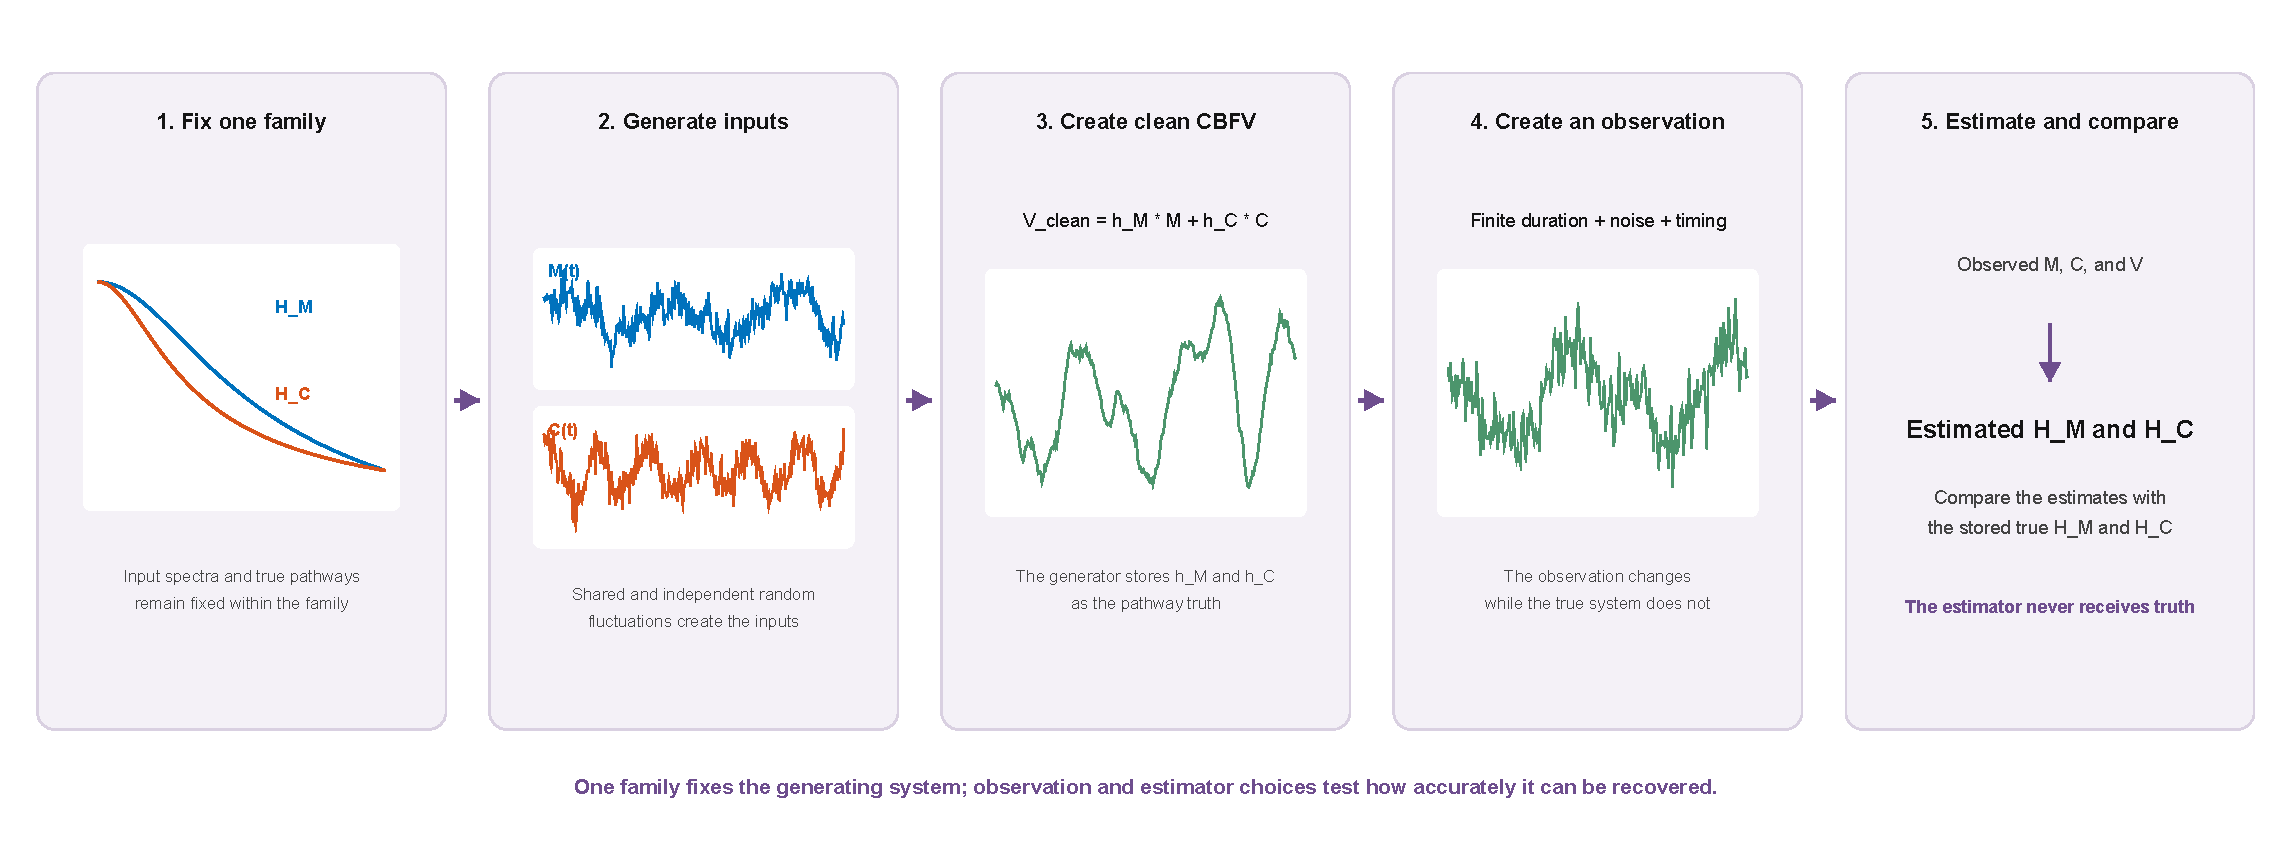
\includegraphics[width=0.96\textwidth]{figures/methods/known_truth_simulation_workflow.pdf}
\end{center}
\sourcefooter{Generated in Python; every displayed trace is a sampled signal realization.}
\end{frame}

\begin{frame}{The estimator is not given the true pathways}
\sectionlabel{Simulation Design}
The generator uses $h_M$ and $h_C$ to create CBFV, but the estimator receives
only the observed $M(t)$, $C(t)$, and $V(t)$. From their Welch spectra it produces
$\widehat H_M(f)$ and $\widehat H_C(f)$ as though the signals were experimental
recordings.

\vspace{0.28cm}
With infinitely long, noiseless, correctly aligned data and a distinguishable
input pair, the correctly specified MISO estimator should approach the generating
pathways. The test is meaningful because finite duration, spectral leakage,
noise, timing error, and input coherence make the estimated spectra imperfect.

\vspace{0.28cm}
SISO has an additional limitation: it intentionally omits one generating input.
When the inputs are related, its pairwise transfer function can differ from the
individual pathway even under otherwise favorable conditions.
\end{frame}

\begin{frame}{Training and validation share truth but not random fluctuations}
\sectionlabel{Simulation Design}
For every family, the program generates two independent baseline realizations
using the same family parameters and the same true $h_M$ and $h_C$. Their random
MAP and $\PETCOtwo$ fluctuations differ.

\vspace{0.16cm}
\begin{equationcallout}
\[
\text{fixed family truth}
\longrightarrow
\begin{cases}
\text{training realization: fit }\widehat H_M,\widehat H_C,\\
\text{validation realization: test prediction on new signals.}
\end{cases}
\]
\end{equationcallout}

\vspace{0.10cm}
Pathway-accuracy outcomes compare the training estimates directly with the stored
true frequency responses. The separate validation realization supports an
additional out-of-sample prediction check without creating a second family.
\end{frame}

\begin{frame}{A family, observation, and estimator setting are different units}
\sectionlabel{Simulation Design}
\fontsize{10.9}{13.2}\selectfont
\begin{tabular}{p{0.21\textwidth}p{0.71\textwidth}}
\toprule
\textbf{Unit} & \textbf{Meaning in the simulation}\\
\midrule
Family & One fixed input structure and pair of true MAP and $\PETCOtwo$ pathways, with independent training and validation realizations. The family is the statistical unit.\\[0.10cm]
Observation & A different way of recording the same family: duration, output noise, input measurement noise, or timing alignment may change while truth remains fixed.\\[0.10cm]
Estimator setting & A different analysis of the same observation, such as Welch window length, overlap, or ridge value.\\
\bottomrule
\end{tabular}

\vspace{0.12cm}
Welch segments, frequency bins, and repeated observations are not counted as
independent families.
\end{frame}

\begin{frame}{Read the family figure as three pairs of questions}
\sectionlabel{Simulation Design}
\fontsize{10.4}{12.9}\selectfont
\begin{tabular}{p{0.09\textwidth}p{0.23\textwidth}p{0.56\textwidth}}
\toprule
\textbf{Panels} & \textbf{Relationship} & \textbf{Question answered}\\
\midrule
A--B & Inputs and output in time & What MAP and $\PETCOtwo$ signals enter the system, and what clean/noisy CBFV signal leaves it?\\[0.10cm]
C--D & Inputs and output in frequency & Where is spectral power available in MAP and $\PETCOtwo$, and where does the resulting CBFV power appear?\\[0.10cm]
E--F & Generating truth and input diagnostic & What did each input pathway contribute to CBFV, and how coherent were the two inputs with each other?\\
\bottomrule
\end{tabular}

\vspace{0.30cm}
Panels A, C, and F describe the \emph{inputs}; panels B and D describe the
\emph{output}; panel E connects each input to its known output contribution.
Transfer-function gain and phase are intentionally shown in the next figure,
not hidden inside this signal-anatomy figure.
\end{frame}

\begin{frame}{One simulated family shows inputs, output, truth, and input coherence}
\sectionlabel{Simulation Design}
\begin{center}
  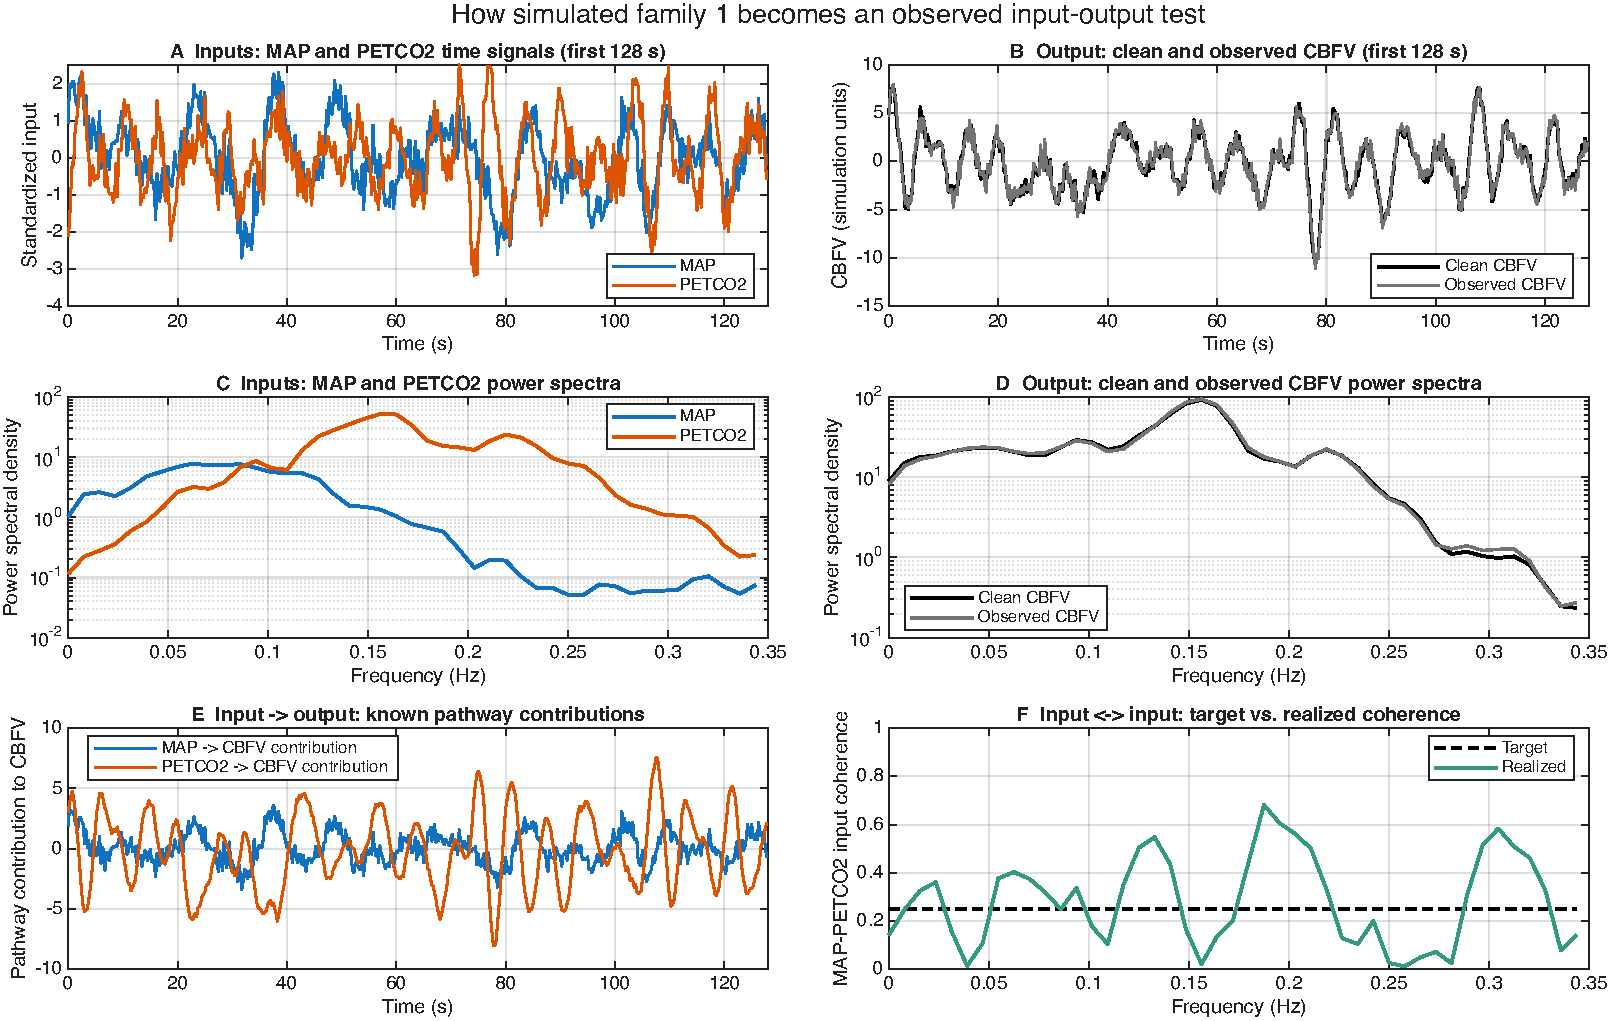
\includegraphics[height=0.59\textheight]{figures/proof250/G01_P02_example_family.pdf}
\end{center}
\proofnote
\end{frame}

\begin{frame}{Panels E and F validate different parts of the generator}
\sectionlabel{Simulation Design}
\textbf{Panel E is input $\rightarrow$ output.} It shows the known filtered MAP
and $\PETCOtwo$ contributions, $V_M(t)$ and $V_C(t)$. These are not raw inputs
and are not estimated transfer functions. Their sample-by-sample sum is clean
CBFV:

\[
V_{\mathrm{clean}}(t)=V_M(t)+V_C(t).
\]

\vspace{0.18cm}
\textbf{Panel F is input $\leftrightarrow$ input.} It compares the configured
MAP-$\PETCOtwo$ coherence target with the coherence realized from one finite
record. It contains no CBFV and therefore does not measure how well either input
explains the output. Variation around the dashed target is expected because the
solid curve is a finite-record Welch estimate.
\end{frame}

\begin{frame}{MAP $\rightarrow$ CBFV gain and phase are evaluated against truth}
\sectionlabel{Simulation Design}
\begin{center}
  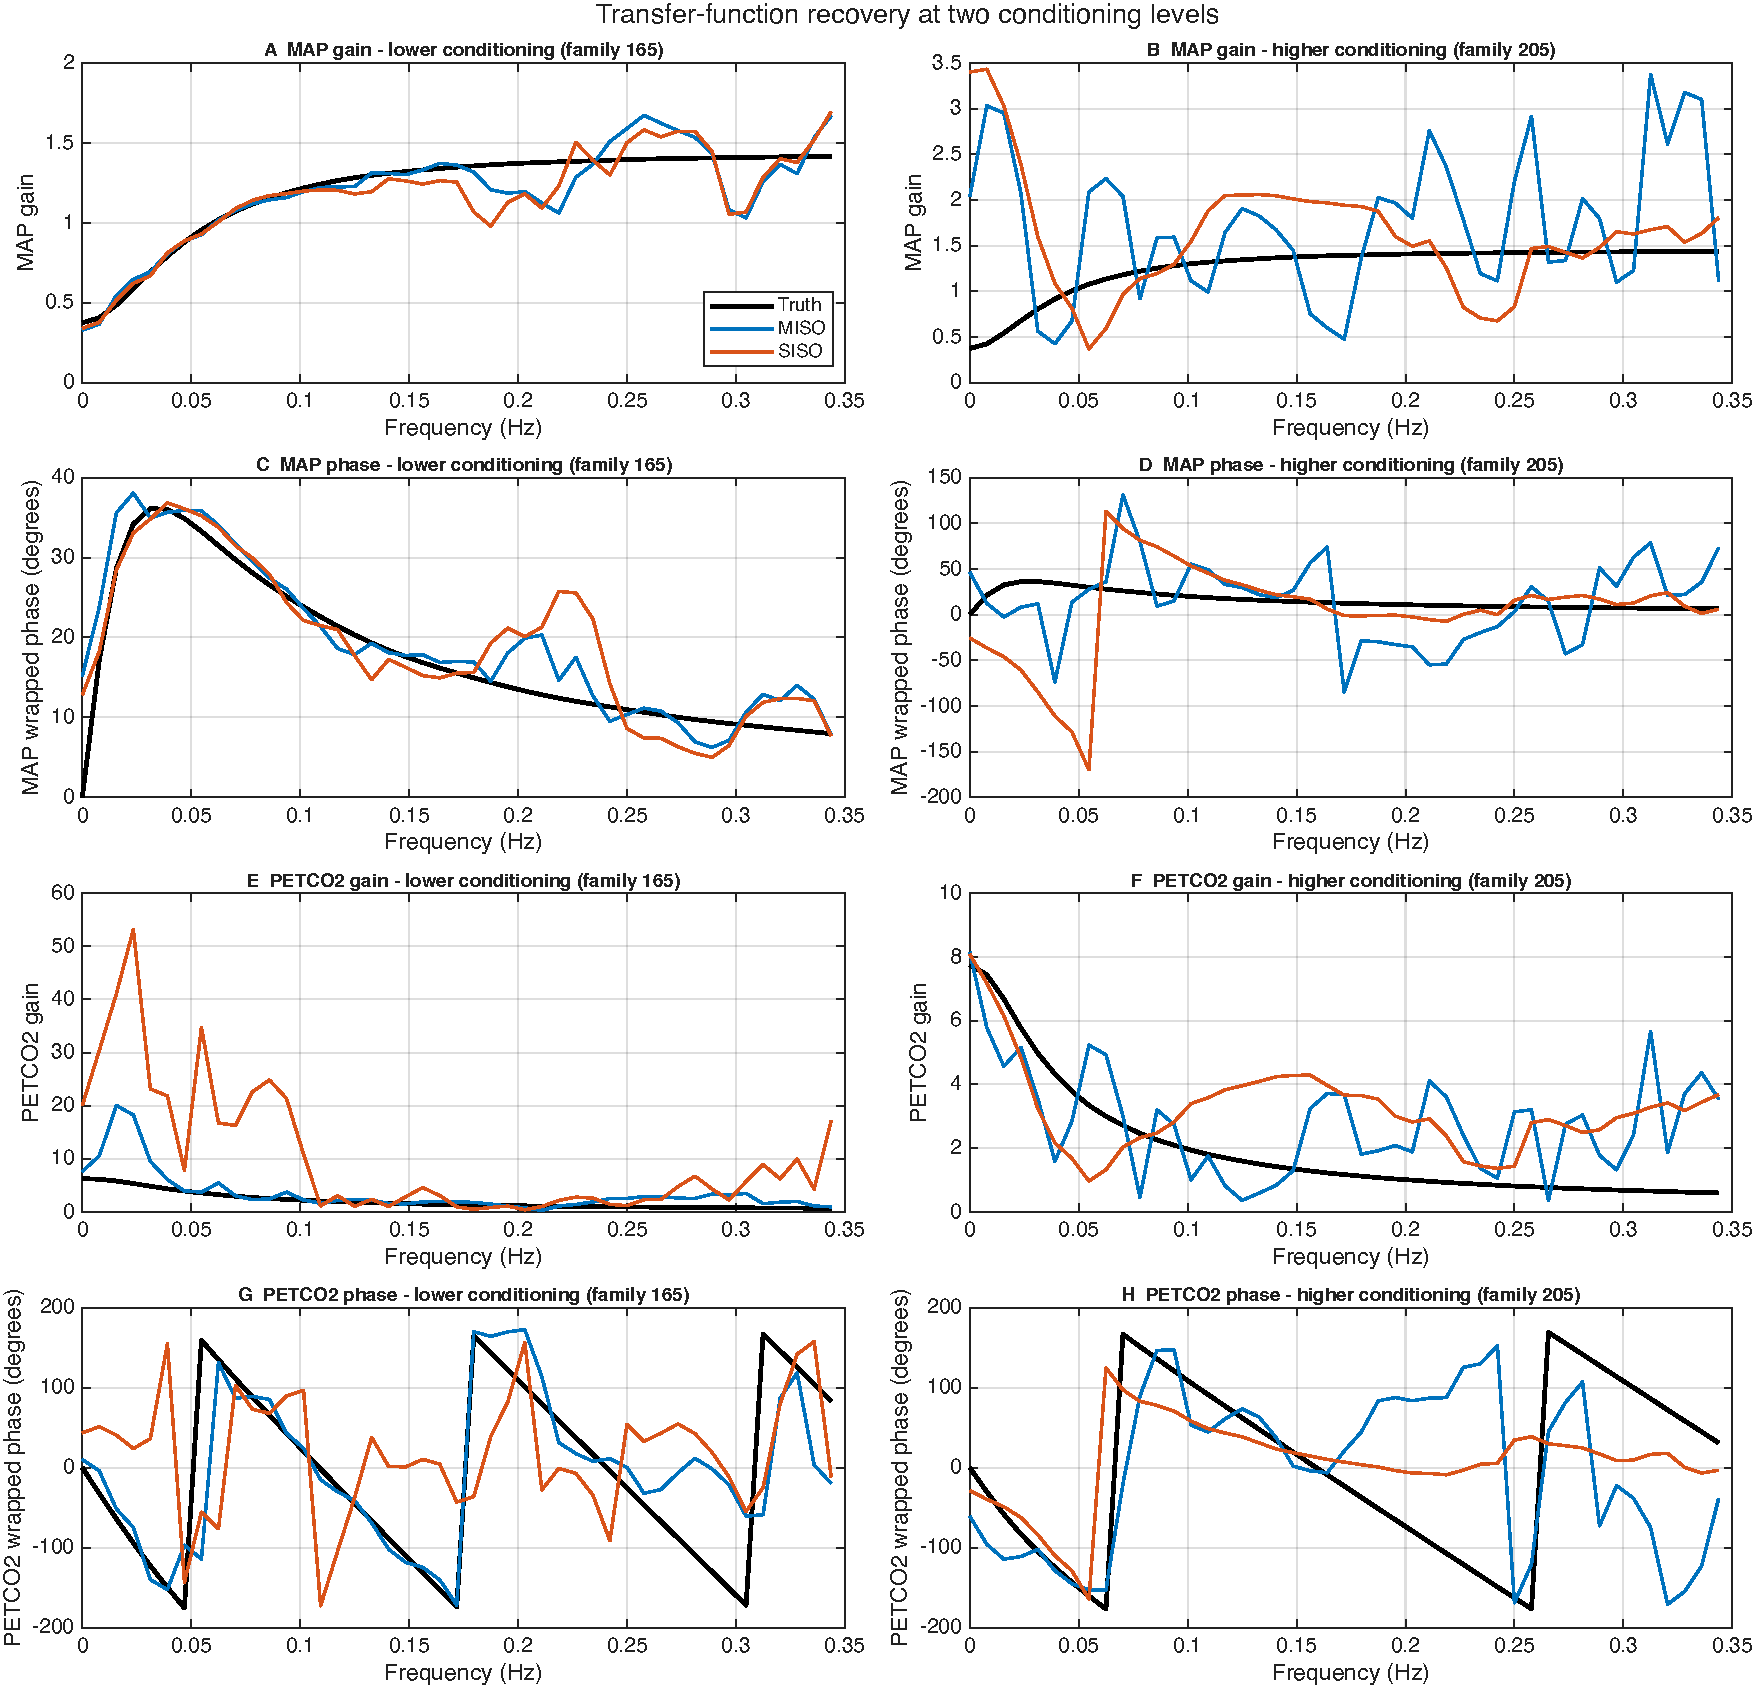
\includegraphics[width=0.60\textwidth,trim=70 425 70 20,clip]{figures/proof250/G01_P03_truth_miso_siso_transfer_functions.pdf}
\end{center}
\sourcefooter{Top row: MAP $\rightarrow$ CBFV gain. Bottom row: MAP $\rightarrow$ CBFV phase. Black is truth; blue is MISO; orange is SISO. Columns compare lower and higher conditioning.}
\end{frame}

\begin{frame}{$\PETCOtwo \rightarrow$ CBFV gain and phase are evaluated against truth}
\sectionlabel{Simulation Design}
\begin{center}
  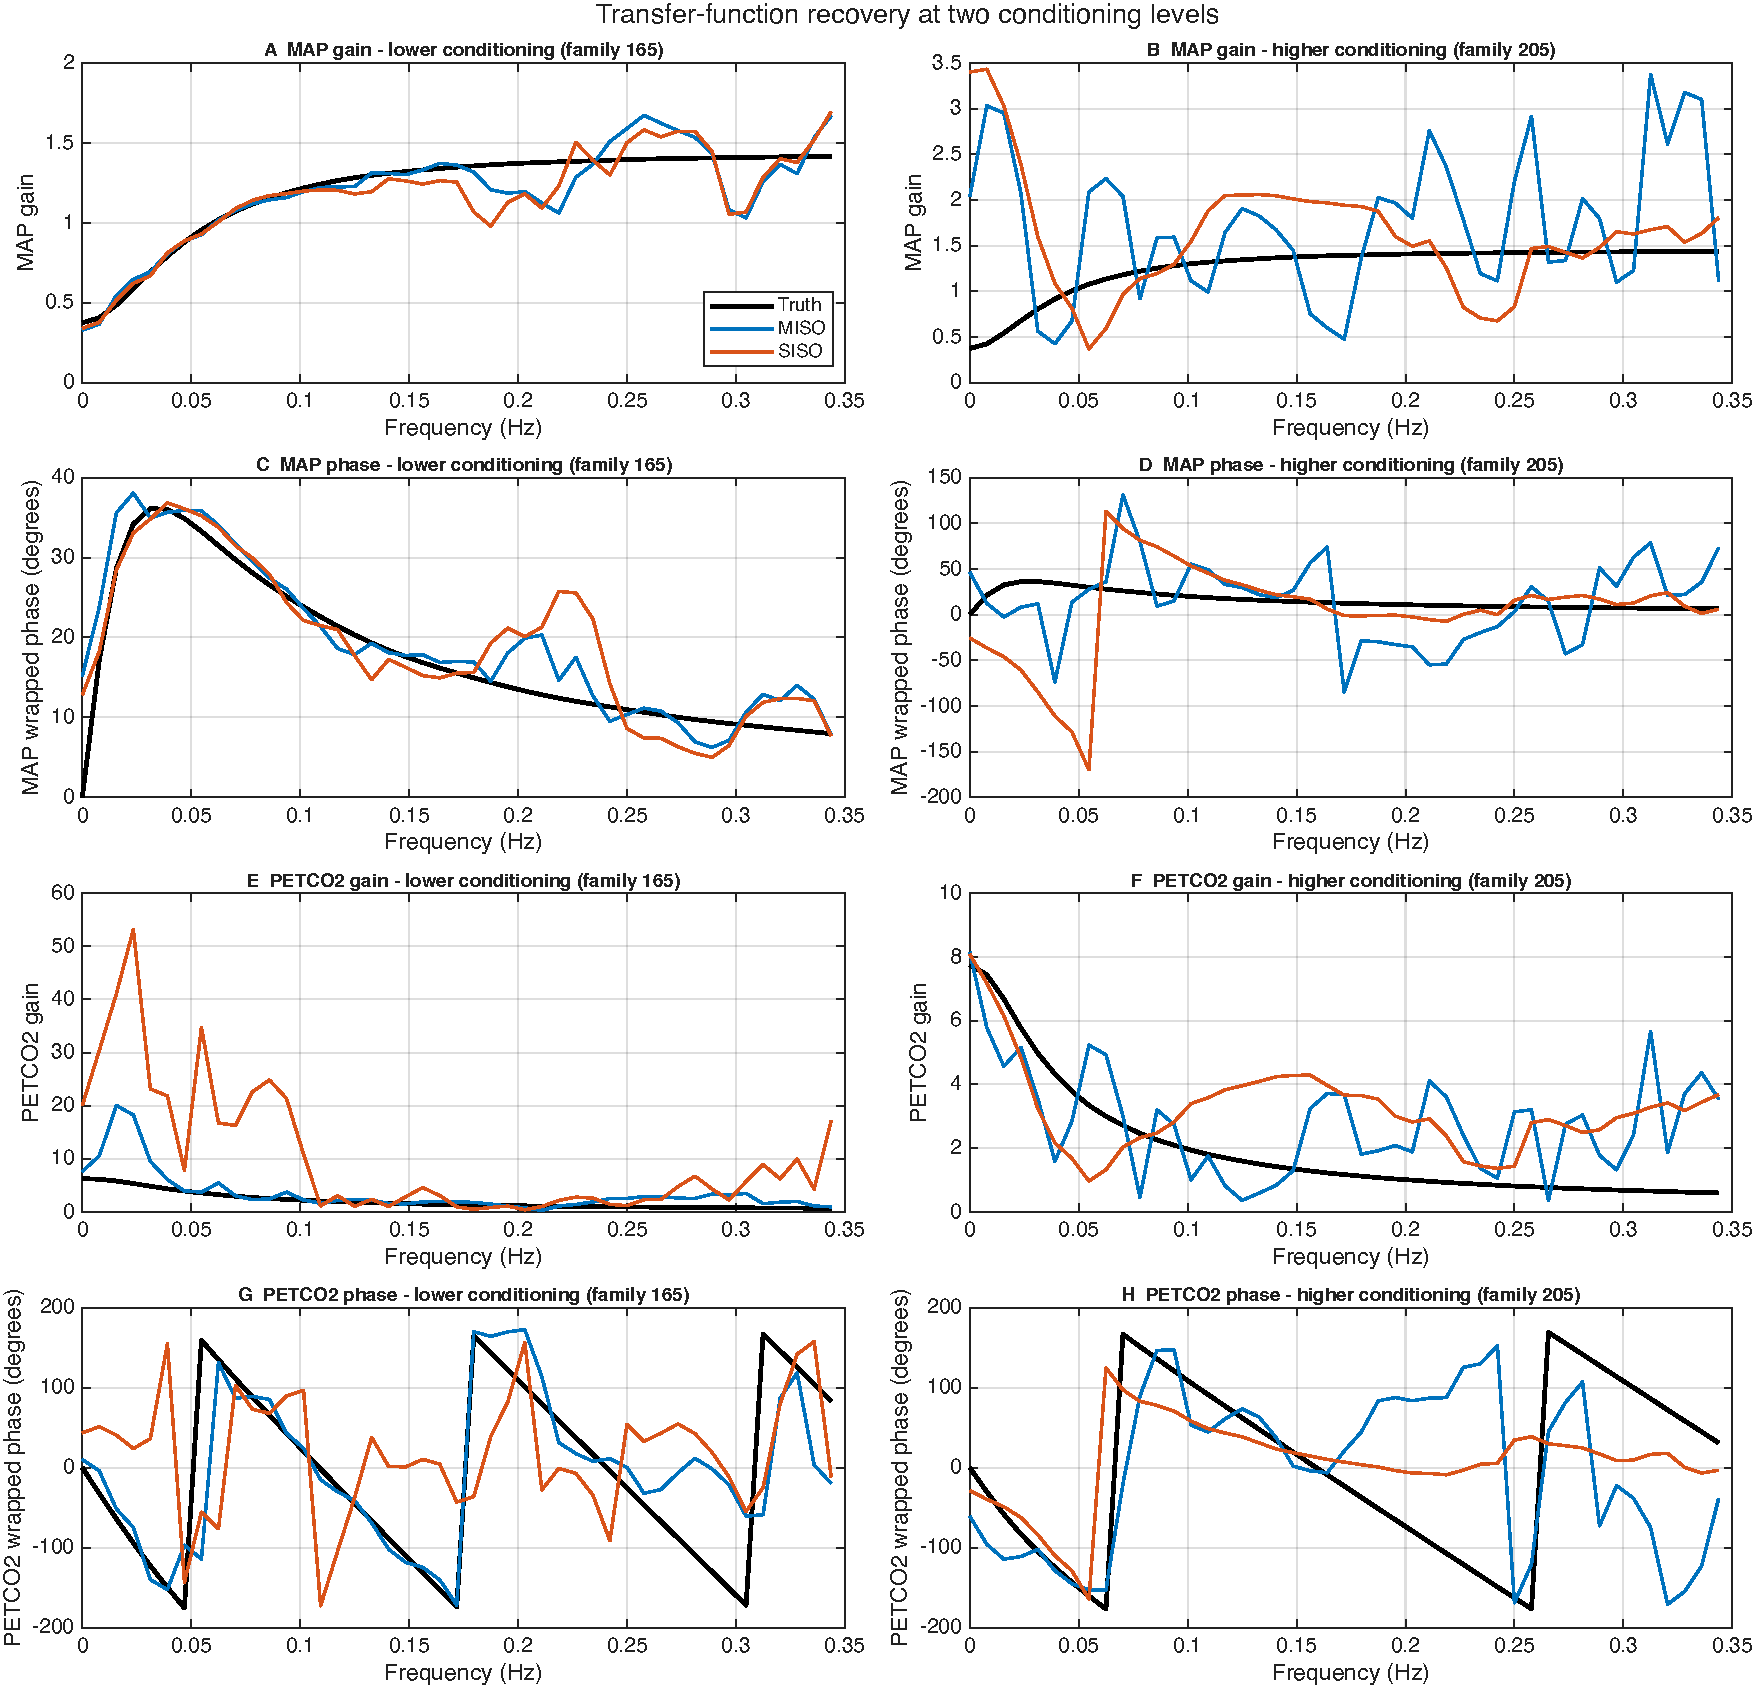
\includegraphics[width=0.53\textwidth,trim=70 20 70 385,clip]{figures/proof250/G01_P03_truth_miso_siso_transfer_functions.pdf}
\end{center}
\sourcefooter{Top row: $\PETCOtwo \rightarrow$ CBFV gain. Bottom row: $\PETCOtwo \rightarrow$ CBFV phase. Black is truth; blue is MISO; orange is SISO. Columns compare lower and higher conditioning.}
\end{frame}

\begin{frame}{Five intrinsic controls define the proof-of-concept families}
\sectionlabel{Simulation Design}
\fontsize{10.3}{12.8}\selectfont
\begin{tabular}{p{0.43\textwidth}p{0.47\textwidth}}
\toprule
\textbf{Assigned family factor} & \textbf{Five configured values}\\
\midrule
Target MAP-$\PETCOtwo$ coherence & 0.05, 0.25, 0.50, 0.75, 0.95\\
Spectral-similarity control & 0, 0.25, 0.50, 0.75, 1\\
$\PETCOtwo$/MAP fluctuation SD ratio & 0.05, 0.25, 0.50, 1, 2\\
$\PETCOtwo$/MAP pathway band-gain ratio & 0.10, 0.50, 1, 2, 4\\
True $\PETCOtwo$ pathway delay & 0, 2.5, 5, 7.5, 10 s\\
\bottomrule
\end{tabular}

\vspace{0.30cm}
MAP and $\PETCOtwo$ pathway time constants remain continuously sampled nuisance
properties over 1--4 s and 2--8 s. They are not forced into categories only to
make the figures look uniform.
\end{frame}

\begin{frame}{Pairwise balance replaces an unnecessary full factorial}
\sectionlabel{Simulation Design}
A complete five-factor design at five levels would require

\[
5^5=3{,}125\ \text{families}.
\]

The proof design instead uses a 25-family base block in which each factor level
appears five times and every pair of factors contains all $5\times5$ level
combinations once. Ten independently generated blocks give

\[
25\ \text{families per block}\times10\ \text{blocks}=250\ \text{families}.
\]

Therefore each assigned level has 50 families and each assigned pairwise cell
has 10. The design protects planned one-factor and two-factor summaries without
claiming to cover all 3,125 five-factor combinations.
\end{frame}

\begin{frame}{Assigned factors and realized characteristics must remain distinct}
\sectionlabel{Simulation Design}
Assigned factors are selected before signal generation and are displayed at
their exact configured values. Realized characteristics are measured from the
longest clean generated record. They can differ slightly from their targets and
are continuous rather than five-valued by definition.

\vspace{0.35cm}
For presentation operating maps, realized input coherence, PSD-shape overlap,
and $\PETCOtwo$ contribution-power share use five fixed intervals:

\[
[0,0.2),\ [0.2,0.4),\ [0.4,0.6),\ [0.6,0.8),\ [0.8,1].
\]

These boundaries were specified before the 250-family results were inspected
and were not moved afterward merely to fill heatmap cells.
\end{frame}

\begin{frame}{Every family receives the same paired observation plan}
\sectionlabel{Simulation Design}
\fontsize{10.2}{12.7}\selectfont
\begin{tabular}{p{0.34\textwidth}p{0.58\textwidth}}
\toprule
\textbf{Experiment} & \textbf{Levels applied to every family}\\
\midrule
Duration by CBFV SNR & Seven durations (256--896 s) crossed with seven output-SNR levels ($\infty$ to 0 dB): 49 observations\\
MAP measurement noise & Seven input-SNR levels at the reference observation\\
$\PETCOtwo$ measurement noise & Seven input-SNR levels at the reference observation\\
$\PETCOtwo$ timing misalignment & $-6,-3,0,3,6$ s at the reference observation\\
\bottomrule
\end{tabular}

\vspace{0.32cm}
The reference observation is 300 s with 15-dB CBFV output SNR, no added input
measurement noise, and no timing misalignment. The plan contains 68 primary
observations per family, producing $250\times68=17{,}000$ primary analyses.
\end{frame}

\begin{frame}{Estimator sensitivity is repeated within each family}
\sectionlabel{Simulation Design}
The primary estimator uses a 128-s Hann window, 50\% overlap, and the common
three-point smoothing kernel $[0.25,\,0.50,\,0.25]$. At least three complete
Welch windows are required.

\vspace{0.40cm}
Sensitivity analyses evaluate ridge values 0.001, 0.01, and 0.1; Welch windows
of 64, 75, 100, 128, and 150 s; overlaps of 25\%, 50\%, and 75\%; and the full
duration-by-window grid. This adds 750 ridge analyses and 10,750 estimator-setting
analyses to the 250-family run.

\vspace{0.40cm}
Because these are repeated analyses of the same underlying families, they
increase the number of computations without increasing the independent sample
size beyond 250.
\end{frame}

\begin{frame}[fragile]{The simulation code mirrors the generating equations}
\sectionlabel{Code Implementation}
\begin{lstlisting}[style=matlabslide]
for family = 1:numberOfFamilies
    [hM,hC] = createTruePathways(family);
    [M,C] = generateRelatedInputs(family);

    Vclean = filter(hM,M) + filter(hC,C);
    [Mobs,Cobs,Vobs] = applyObservationPlan( ...
        M,C,Vclean,duration,noise,timing);

    spectra = welchSpectra(Mobs,Cobs,Vobs);
    Hhat = solveMISO(spectra);
    error = compareWithTruth(Hhat,hM,hC);
end
\end{lstlisting}
\sourcefooter{Conceptual implementation of the simulation workflow. The production project separates these operations into tested generator, observation, spectral-estimation, solver, and metric functions.}
\end{frame}

% =============================================================================
% Section 8
% =============================================================================

\section{Known-truth comparison}
\sectionframe{8}{How the Estimates Are Compared With Truth}{%
The primary outcome compares the complete complex transfer function, while gain
and phase errors explain which part of the estimate changed.}

\begin{frame}{Complex error combines magnitude and phase disagreement}
\sectionlabel{Known-Truth Outcomes}
For an estimated pathway $\widehat H(f)$ and its known truth $H(f)$, the code
averages squared complex distance over the analyzed frequency range and
normalizes by the mean energy of the true transfer function:

\vspace{0.12cm}
\begin{equationcallout}
\[
E_{\mathrm{complex}}
=
\frac{\operatorname{mean}_{f}\left|\widehat H(f)-H(f)\right|^2}
     {\operatorname{mean}_{f}|H(f)|^2}.
\]
\end{equationcallout}

\vspace{0.10cm}
This retains disagreement in both gain and phase. Separate absolute gain and
wrapped-phase errors are also calculated to make the result easier to interpret.
\end{frame}

\begin{frame}{Phase error is evaluated only where the true pathway is defined}
\sectionlabel{Known-Truth Outcomes}
Phase becomes unstable or physically uninformative where true pathway gain is
nearly zero. The implementation therefore evaluates wrapped phase error only at
frequencies where true gain exceeds 5\% of its root-mean-square gain.

\vspace{0.20cm}
\begin{equationcallout}
\[
e_{\phi}(f)=
\angle\!\left[\exp\!\left(i\{\angle\widehat H(f)-\angle H(f)\}\right)\right].
\]
\end{equationcallout}

\vspace{0.20cm}
This returns the principal angular difference rather than treating a $2\pi$
representation change as a large physiological error.
\end{frame}

\begin{frame}{Model advantage expresses the relative error on a log scale}
\sectionlabel{Known-Truth Outcomes}
\fontsize{9.4}{11.6}\selectfont
For the same family and observation, SISO and MISO error are converted into a
model-advantage value:

\vspace{0.20cm}
\begin{equationcallout}
\[
\Amodel=\log_{10}\!\left(
\frac{E_{\mathrm{SISO}}+\epsilon}
     {E_{\mathrm{MISO}}+\epsilon}\right),
\qquad \epsilon=10^{-12}.
\]
\end{equationcallout}

\vspace{0.02cm}
\begin{center}
{\color{Co2Orange}\textbf{$\Amodel<0$: SISO has lower error}}
\qquad $\Amodel=0$: equal error \qquad
{\color{MapBlue}\textbf{$\Amodel>0$: MISO has lower error}}
\end{center}

\vspace{0.02cm}
$A_{\mathrm{model}}=0.30$ means the SISO error is about twice the MISO error;
$A_{\mathrm{model}}=1$ means it is ten times larger. Always show absolute SISO
and MISO errors too: a favorable ratio can coexist with poor performance by
both models.
\end{frame}

\begin{frame}{Aggregation preserves the family as the independent unit}
\sectionlabel{Known-Truth Outcomes}
Each displayed group or heatmap cell is summarized across families, not across
Welch segments or frequency bins treated as independent repetitions. Exported
source data retain the mean, standard deviation, valid family count, total group
count, standard error, confidence interval, and probability values when
inference is performed.

\vspace{0.45cm}
The presentation display threshold is five valid families. Cells below this
threshold remain gray and receive no mean color. Five families permit a
descriptive calculation; they do not by themselves provide strong publication
evidence. Frequency-resolved plots keep the native Welch frequency bins rather
than rebinned frequencies.
\end{frame}

% =============================================================================
% Section 9
% =============================================================================

\section{Proof-of-concept results}
\sectionframe{9}{Audited 250-Family Proof-of-Concept Results}{%
The run verifies the design and demonstrates the expected MISO accuracy--stability
tradeoff. These results guide the final paper design rather than replace it.}

\begin{frame}{The proof-of-concept run completed as designed}
\sectionlabel{Simulation Audit}
\begin{tabular}{p{0.48\textwidth}r}
\toprule
\textbf{Completed quantity} & \textbf{Count}\\
\midrule
Independent simulated families & 250\\
Complete 25-family balanced blocks & 10\\
Primary observation analyses & 17,000\\
Ridge analyses & 750\\
Estimator-setting analyses & 10,750\\
Audited metric-condition support checks & 748\\
Numerical runtime & 21.3 min\\
\bottomrule
\end{tabular}

\vspace{0.35cm}
All 14 core execution checks passed. All 25 marginal level checks and all 250
assigned pairwise-cell checks passed. No audited whole-range metric value was
silently discarded as nonfinite.
\proofnote
\end{frame}

\begin{frame}{Assigned controls were reproduced by the generator}
\sectionlabel{Generator Validation}
\begin{center}
  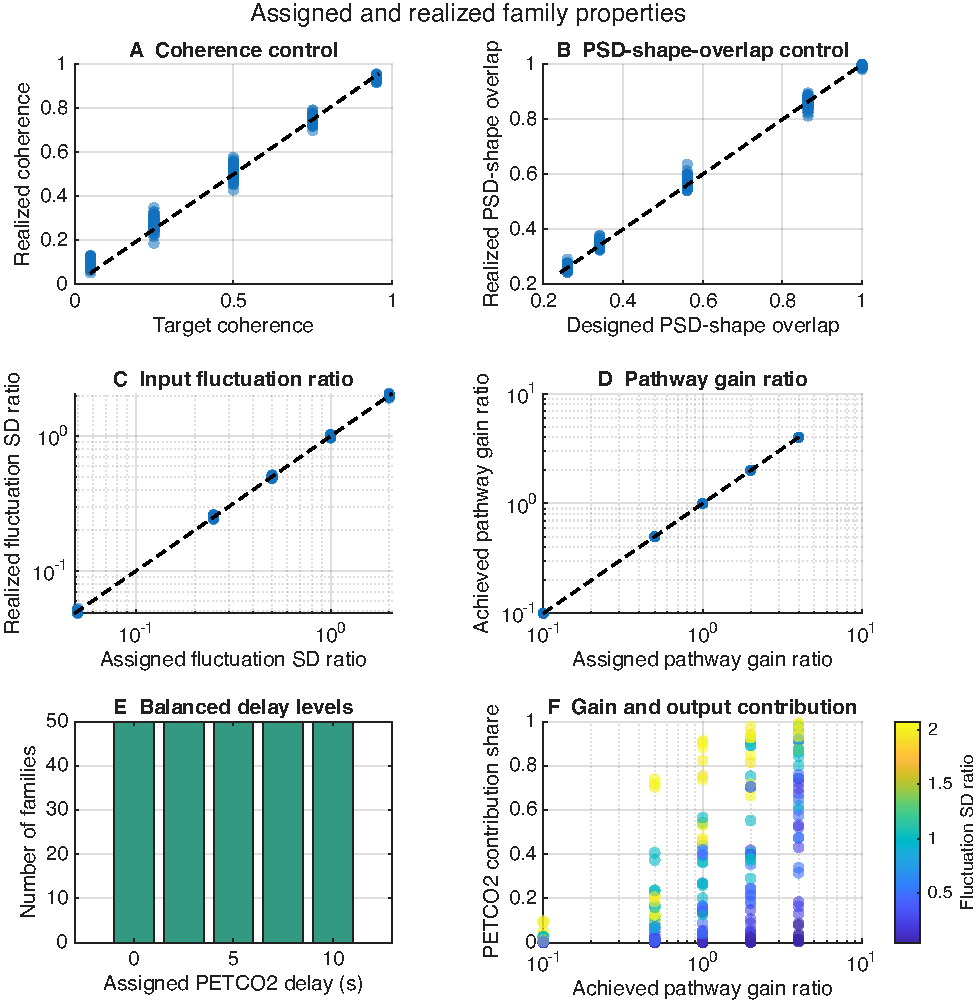
\includegraphics[height=0.69\textheight]{figures/proof250/G02_P01_target_realized_validation.pdf}
\end{center}
\proofnote
\end{frame}

\begin{frame}{Balanced checkpoints support using 250 families for this deck}
\sectionlabel{Simulation Audit}
The design contains natural complete-block checkpoints at 125, 200, and 250
families. Across the six reference-condition complex, gain, and phase
model-advantage outcomes, the largest absolute difference from the final
250-family mean was 0.0339 at 125 families and 0.0169 at 200 families.

\vspace{0.45cm}
These are descriptive stability checks rather than additional hypothesis tests.
They show that the main proof-of-concept averages were not being driven by the
last few families, while still leaving the larger 1,000-family profile necessary
for stronger cell support and final publication-level modeling.
\proofnote
\end{frame}

\begin{frame}{At the reference condition, MISO had lower mean error}
\sectionlabel{Reference-Condition Result}
\begin{center}
  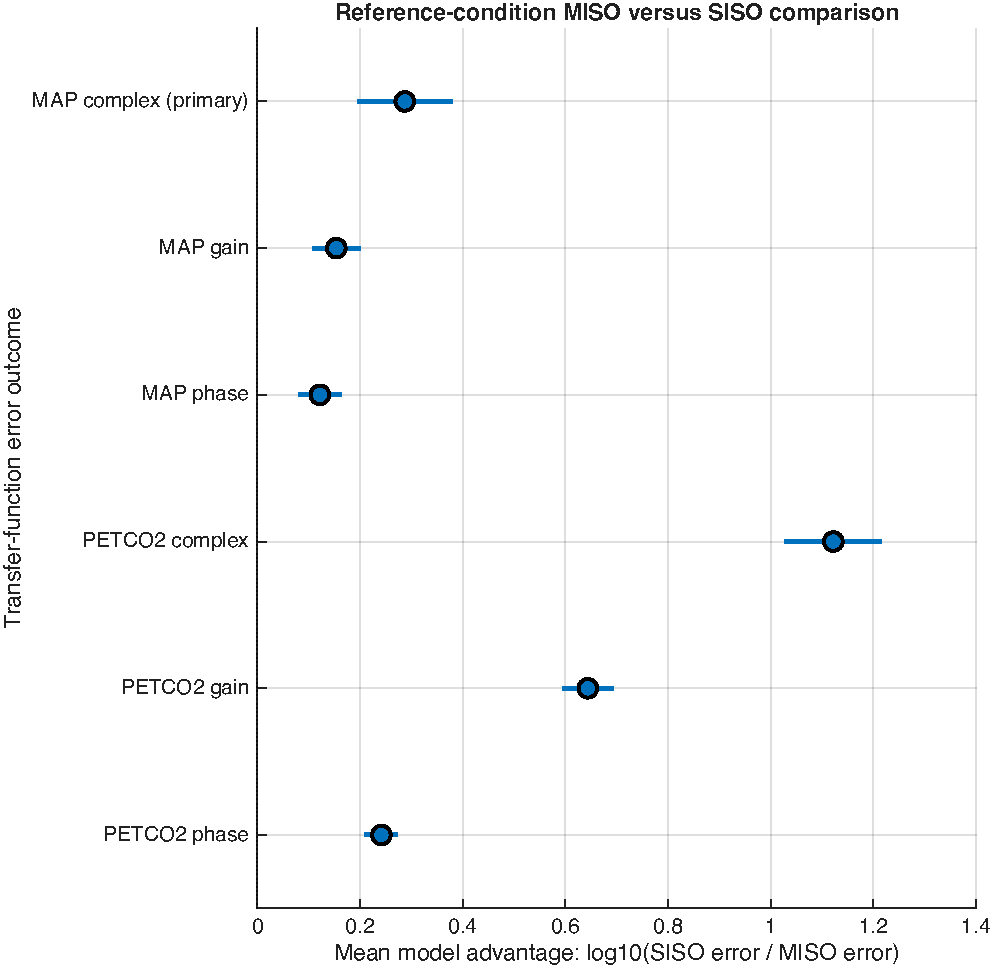
\includegraphics[height=0.63\textheight]{figures/proof250/G02_P03_reference_model_statistics.pdf}
\end{center}
\sourcefooter{Means and 95\% confidence intervals across 250 families. Black rings mark the reported comparison after the stated adjustment family. Model advantage is $\log_{10}(E_{\mathrm{SISO}}/E_{\mathrm{MISO}})$.}
\end{frame}

\begin{frame}{The reference result was larger for the $\PETCOtwo$ pathway}
\sectionlabel{Reference-Condition Result}
At 300 s, 15-dB CBFV output SNR, and no input noise or timing shift, mean MAP
complex model advantage was 0.287 (95\% CI 0.194 to 0.380). This corresponds to
an approximately 1.94-fold geometric SISO-to-MISO error ratio.

\vspace{0.35cm}
Mean $\PETCOtwo$ complex model advantage was 1.122 (95\% CI 1.028 to 1.216),
corresponding to an approximately 13.25-fold geometric error ratio. Gain and
phase comparisons were also positive on average for both pathways.

\vspace{0.35cm}
This establishes a proof-of-concept average difference, not a claim that MISO
is better in every family. The next analyses examine where that average changes.
\proofnote
\end{frame}

\begin{frame}{Very high input coherence changes the MAP tradeoff}
\sectionlabel{Input Identifiability Result}
\begin{center}
  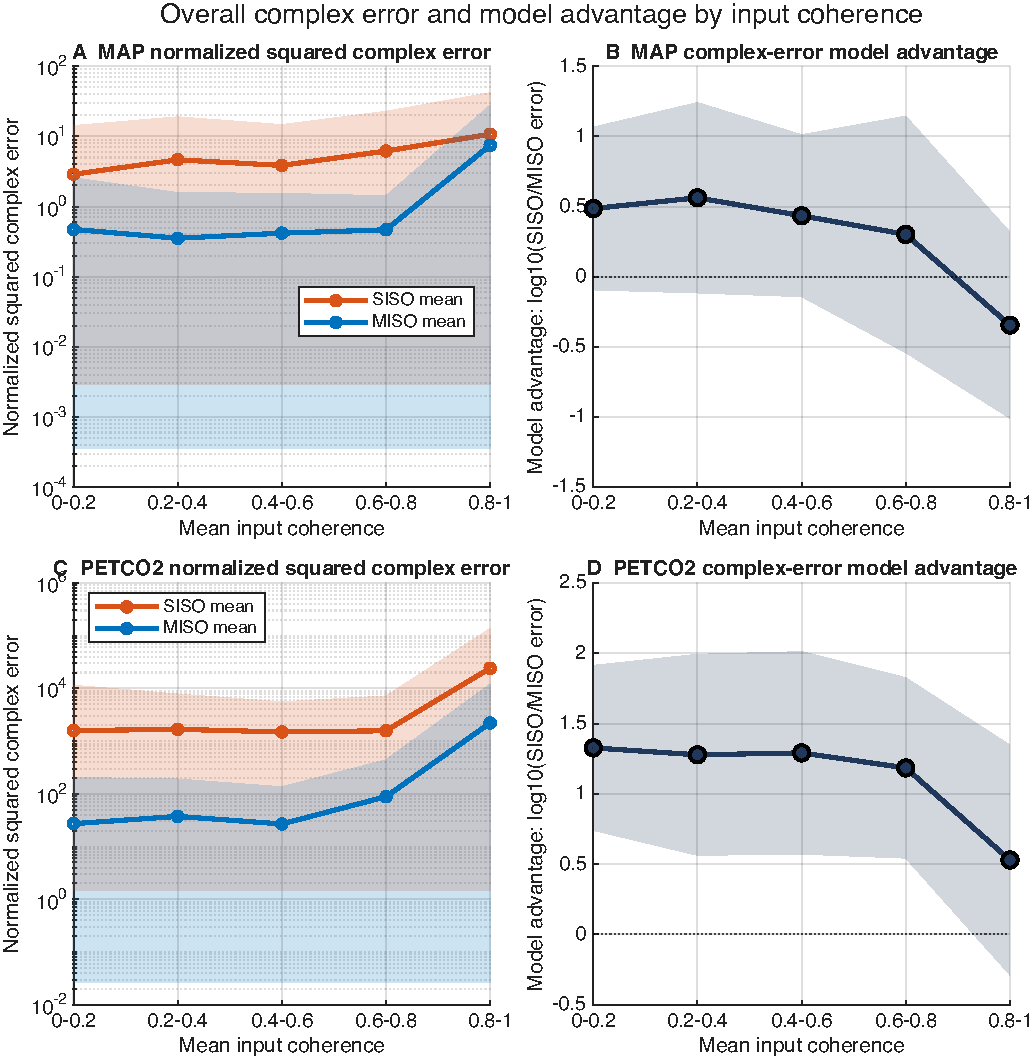
\includegraphics[height=0.63\textheight]{figures/proof250/G07_input_coherence_overall_complex_error.pdf}
\end{center}
\sourcefooter{Families are grouped by prespecified intervals of realized mean input coherence. Curves show across-family means; shaded regions show SD.}
\end{frame}

\begin{frame}{The highest-coherence group illustrates the stability limit}
\sectionlabel{Input Identifiability Result}
MAP model advantage remained positive through the 0.6--0.8 realized-coherence
group, but the 0.8--1.0 group had a mean advantage of $-0.346$ (95\% CI $-0.534$
to $-0.157$). Its geometric SISO-to-MISO error ratio was 0.45, indicating lower
MAP SISO error on average in that group.

\vspace{0.35cm}
The $\PETCOtwo$ advantage also decreased at the highest coherence but remained
positive on average: 0.529 (95\% CI 0.297 to 0.762). This difference between
pathways is important. Poor identifiability does not have to affect both true
pathways in the same way because their excitation and pathway gains also differ.
\proofnote
\end{frame}

\begin{frame}{Condition number connects coherence with known-truth error}
\sectionlabel{Input Identifiability Result}
\begin{center}
  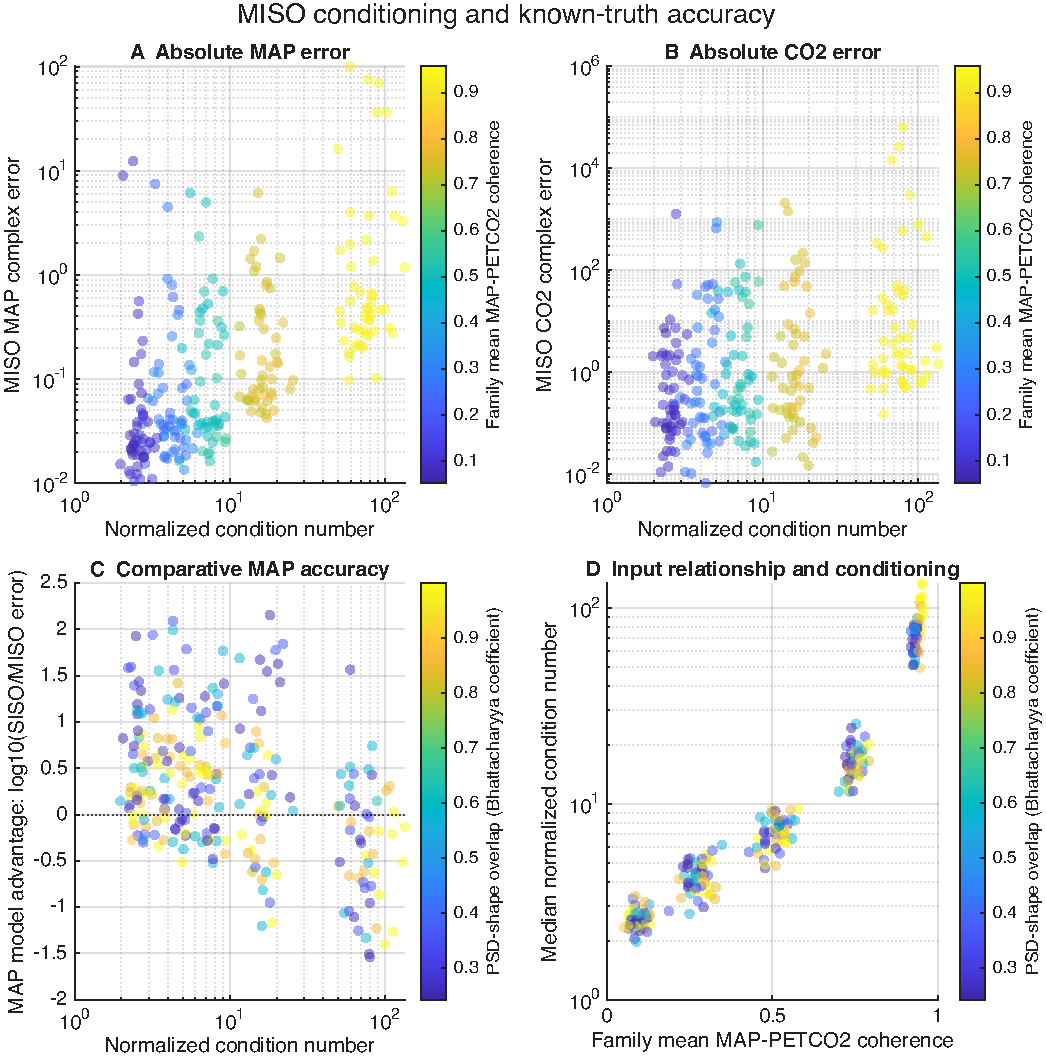
\includegraphics[height=0.54\textheight]{figures/proof250/G07_conditioning_diagnostics.pdf}
\end{center}
\sourcefooter{Each point represents one family at the reference observation. Conditioning is calculated after scaling the inputs to unit spectral power.}
\end{frame}

\begin{frame}{Excitation and pathway gain must be interpreted together}
\sectionlabel{Pathway Excitation Result}
\begin{center}
  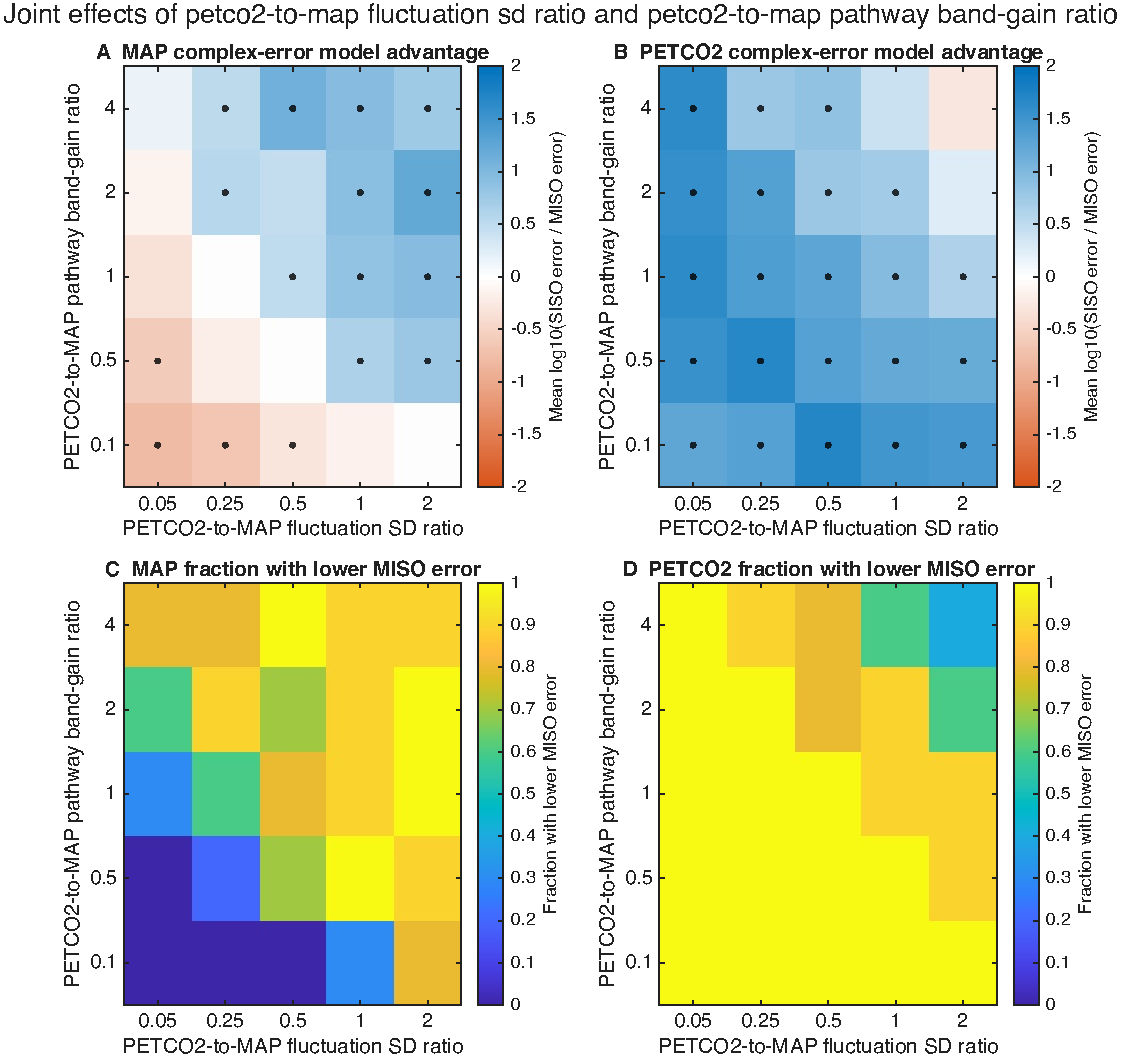
\includegraphics[height=0.59\textheight]{figures/proof250/G18_fluctuation_by_pathway_gain.pdf}
\end{center}
\sourcefooter{Axes use exact assigned values; each $5\times5$ pairwise cell contains 10 families. Black dots mark adjusted $P<0.05$.}
\end{frame}

\begin{frame}{Weak $\PETCOtwo$ influence can limit the MAP benefit}
\sectionlabel{Pathway Excitation Result}
The joint assigned-factor map separates the strength of $\PETCOtwo$ fluctuations
from the strength of its pathway to CBFV. MAP MISO advantage is weakest, and can
be negative, when both the $\PETCOtwo$ input and its pathway are very weak. In
that region there is little second-pathway influence for MISO to separate, so an
additional coefficient can add finite-record variability without removing much
SISO mixing.

\vspace{0.40cm}
As either the $\PETCOtwo$ fluctuations or pathway gain becomes stronger, MAP
MISO advantage generally increases. The $\PETCOtwo$ pathway shows a broader
positive MISO advantage, but its exact magnitude also changes across the joint
design. This supports interpreting excitation and pathway strength as separate
controls rather than one combined label.
\proofnote
\end{frame}

\begin{frame}{Timing alignment changes the two pathways differently}
\sectionlabel{Observation-Quality Result}
\begin{center}
  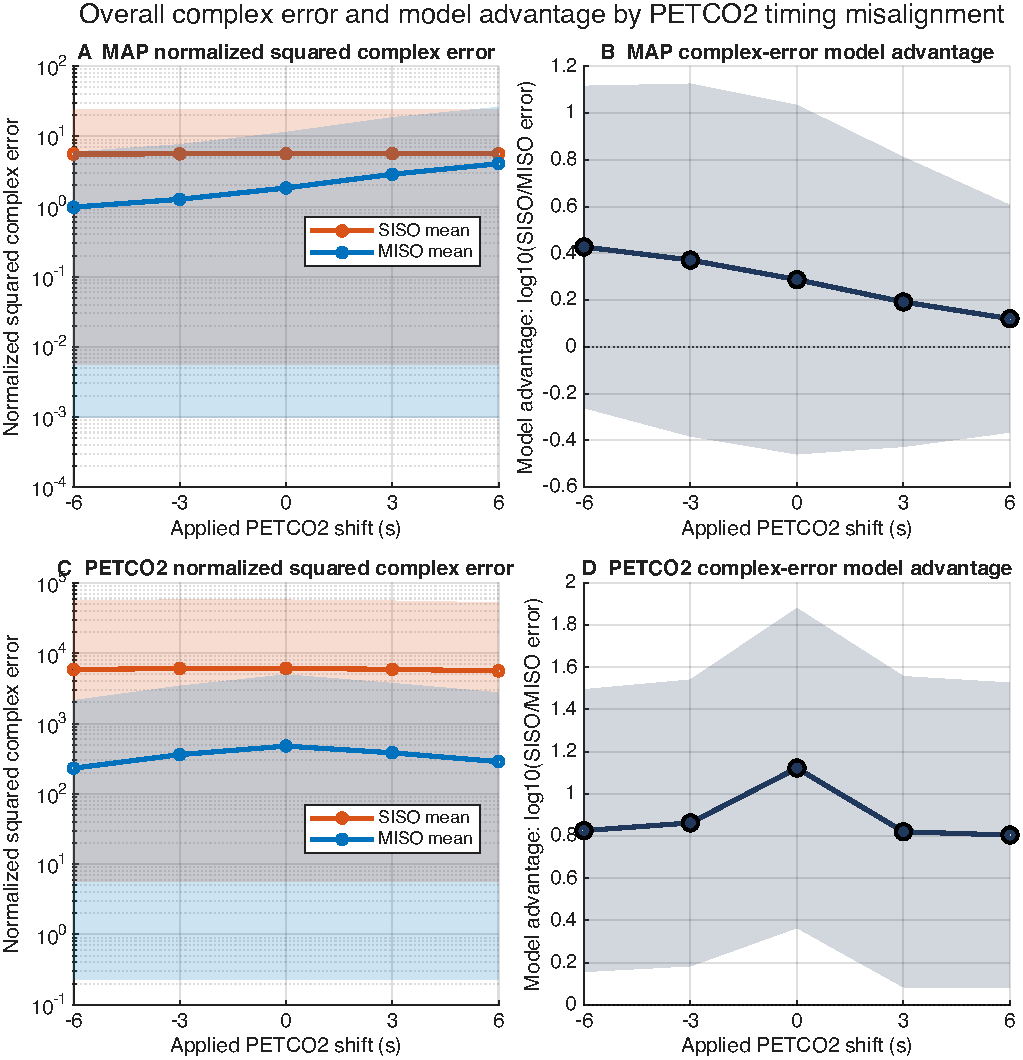
\includegraphics[height=0.53\textheight]{figures/proof250/G13_petco2_timing_misalignment_overall_complex_error.pdf}
\end{center}
\sourcefooter{Each timing shift is applied to the same 250 families at the reference duration and output SNR. Curves show across-family means; shaded regions show SD.}
\end{frame}

\begin{frame}{The timing result is directional rather than a single penalty}
\sectionlabel{Observation-Quality Result}
The $\PETCOtwo$ complex model advantage was largest with no applied timing shift
(1.122) and decreased to approximately 0.80--0.86 after shifts of three or six
seconds in either direction. MAP advantage changed asymmetrically: it was 0.287
at zero shift, 0.120 at $+6$ s, and 0.427 at $-6$ s.

\vspace{0.40cm}
This asymmetry is consistent with timing error interacting with the families'
true $\PETCOtwo$ delays rather than acting as one uniform amount of noise. A
recording's alignment choice can therefore change which complex pathway is
easier to recover and should be treated as part of the model specification.
\proofnote
\end{frame}

\begin{frame}{Longer records generally strengthen the advantage}
\sectionlabel{Finite-Record Result}
\begin{center}
  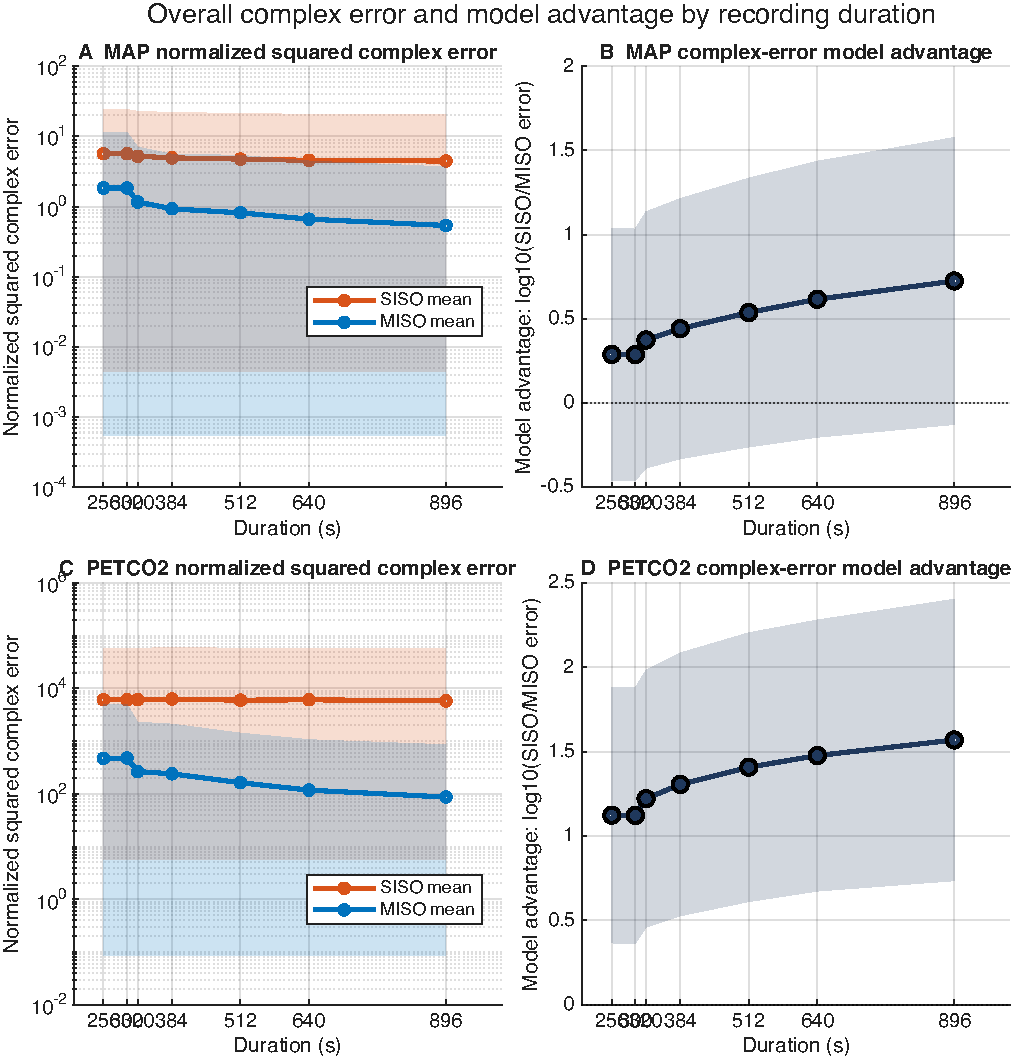
\includegraphics[height=0.63\textheight]{figures/proof250/G03_duration_overall_complex_error.pdf}
\end{center}
\sourcefooter{Durations use exact configured values. All curves use 15-dB CBFV output SNR and the primary 128-s, 50\%-overlap Welch estimator.}
\end{frame}

\begin{frame}{Duration and Welch window length form one estimator tradeoff}
\sectionlabel{Finite-Record Result}
\begin{center}
  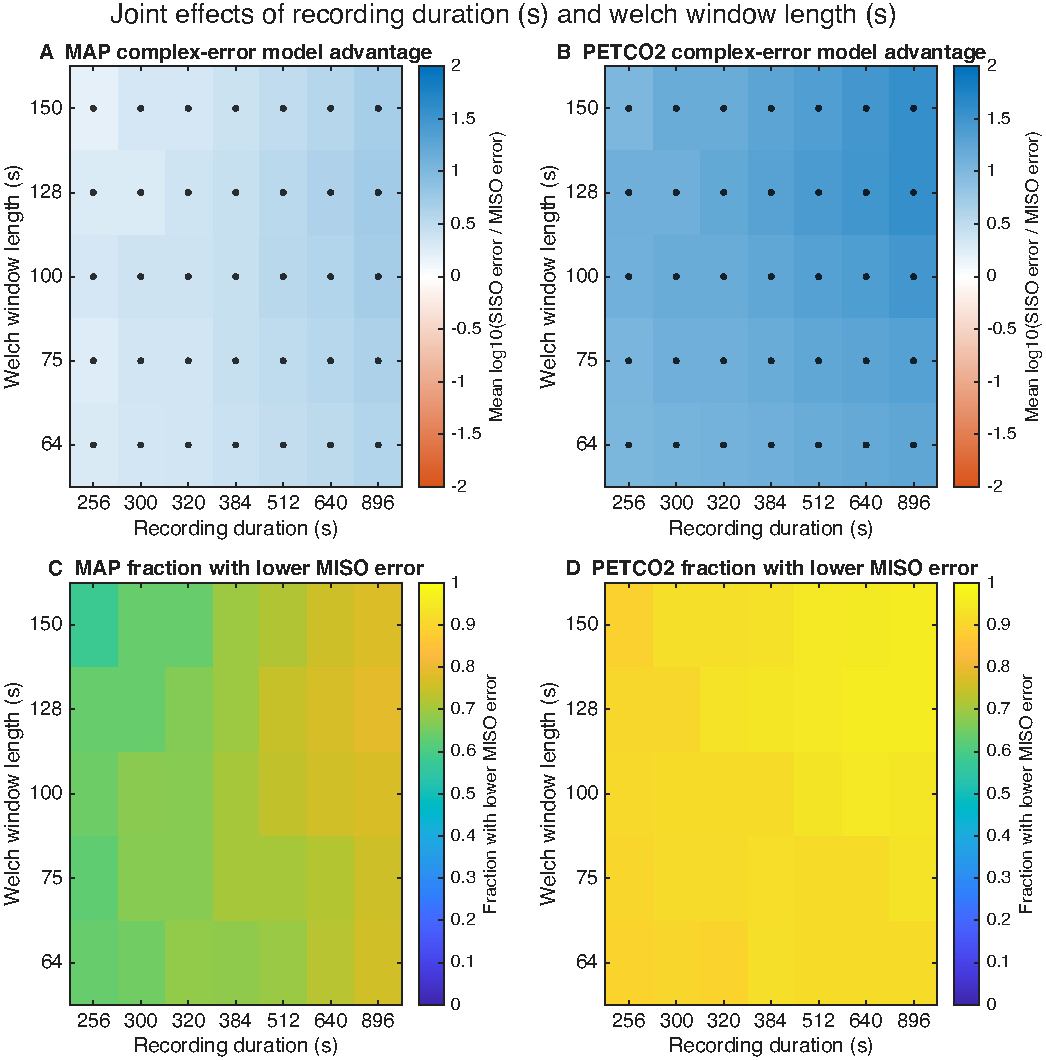
\includegraphics[height=0.59\textheight]{figures/proof250/G19_duration_by_welch_window.pdf}
\end{center}
\sourcefooter{Axes use exact configured values. Each cell summarizes the same 250 families; black dots mark adjusted $P<0.05$.}
\end{frame}

\begin{frame}{The interaction map supports an intuitive interpretation}
\sectionlabel{Finite-Record Result}
Longer recordings generally increase the amount of information available to
both models and increase the fraction of families in which MISO has lower
complex error. Window length modifies this result because it controls the
balance between frequency resolution and the number of segment-level estimates
that can be averaged.

\vspace{0.40cm}
The $\PETCOtwo$ pathway shows a broad MISO advantage across the tested
duration-window grid. The MAP pathway shows more gradual improvement with
duration and greater dependence on window choice. This difference reinforces
that estimator settings should not be selected only from one pathway's behavior.
\proofnote
\end{frame}

% =============================================================================
% Section 10
% =============================================================================

\section{Limits and transition to the paper}
\sectionframe{10}{What the Proof of Concept Establishes--and What It Does Not}{%
The run supports the workflow and the main tradeoff, while also identifying
design decisions that must be made before the final paper simulation.}

\begin{frame}{Realized bins reveal where the current design is sparse}
\sectionlabel{Proof-of-Concept Limitations}
\begin{center}
  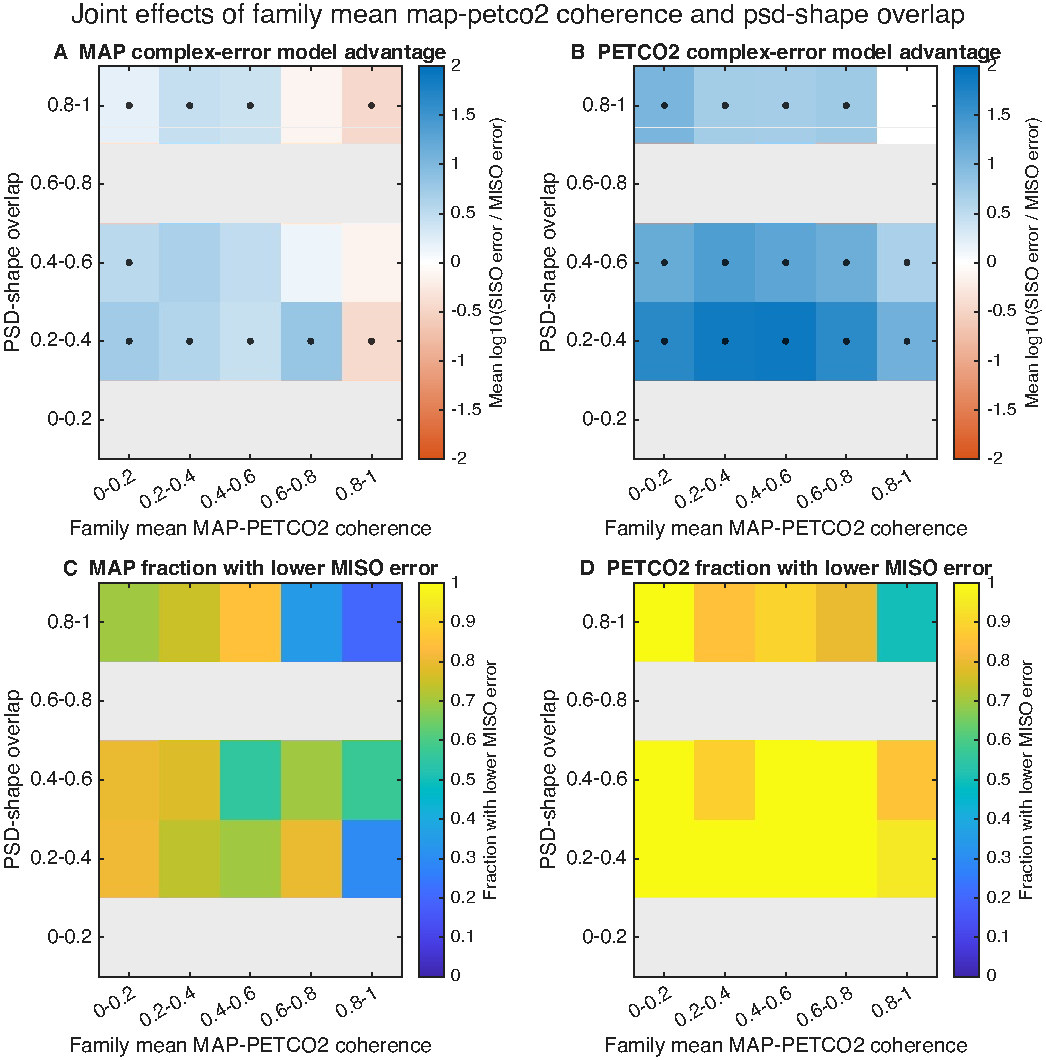
\includegraphics[height=0.67\textheight]{figures/proof250/G17_coherence_by_psd_overlap.pdf}
\end{center}
\sourcefooter{Gray cells contain fewer than five valid families. The fixed realized-value boundaries were not moved after seeing occupancy.}
\end{frame}

\begin{frame}{The gray cells are information about support, not missing results}
\sectionlabel{Proof-of-Concept Limitations}
Realized coherence occupied the five bins almost evenly: 51, 49, 50, 50, and 50
families. Realized PSD-shape overlap was uneven: 0, 100, 45, 5, and 100. Across
the three audited two-dimensional realized-characteristic grids, 43 of 75 cells
met the five-family display threshold and 13 were empty.

\vspace{0.40cm}
The unsupported cells remain gray because the proof design did not generate
enough families there. Filling them by changing bin boundaries after seeing the
data would make the figure look more complete without adding information. These
maps are therefore descriptive and should not be treated as precise boundaries
of an operating region.
\proofnote
\end{frame}

\begin{frame}{The 1,000-family run is a planned extension, not a simple rerun}
\sectionlabel{Transition to the Final Paper}
Repeating the 25-family balanced block 40 times would provide 1,000 families,
40 families per assigned pairwise cell, and greater support for continuous
models or finer descriptive grouping. Before that run, the following choices
should be specified prospectively:

\vspace{0.25cm}
\begin{itemize}
  \item final continuous-bin boundaries and minimum cell size;
  \item which interactions are primary, secondary, or supplemental;
  \item whether spectral-similarity coverage should be expanded;
  \item the primary endpoint and multiplicity families; and
  \item which family-level continuous regression models will support formal claims.
\end{itemize}

The larger sample should increase evidence, not replace the design decisions
revealed by the proof of concept.
\end{frame}

\begin{frame}{The current conclusion is methodological and conditional}
\sectionlabel{Proof-of-Concept Synthesis}
The 250-family run shows that MISO can recover both known pathways more accurately
on average under the reference observation, with an especially large average
advantage for the $\PETCOtwo$ pathway. It also shows why that conclusion cannot
be reduced to ``MISO is better.'' MAP accuracy can favor SISO when the inputs are
extremely coherent, and MISO benefit changes with excitation, pathway gain,
timing, record duration, and estimator settings.

\vspace{0.45cm}
The next scientific step is to finalize the paper-scale design using these audit
findings, run the 1,000-family profile, and only then place the cognitively normal
human recordings within the supported simulated operating space.
\end{frame}

% =============================================================================
% Methods and reference appendix
% =============================================================================

\section{Methods and reference appendix}
\sectionframe{A}{Methods and Reference Appendix}{%
The essential equations belong in the paper's main Methods. The expanded
derivations, assumptions, and source bank are retained here to stage the
supplement and make every design choice traceable.}

\begin{frame}{The paper and supplement should overlap where the math carries meaning}
\sectionlabel{Appendix Road Map}
\fontsize{10.4}{13.0}\selectfont
\begin{columns}[T,onlytextwidth]
\begin{column}{0.46\textwidth}
\textbf{Keep visible in the main paper}
\begin{itemize}
  \item the $2\times2$ spectral model;
  \item the shared/independent input construction;
  \item both true pathways and the observation plan; and
  \item complex error plus signed model advantage.
\end{itemize}
\end{column}
\begin{column}{0.48\textwidth}
\textbf{Expand in the supplement}
\begin{itemize}
  \item SISO contamination and the explicit MISO solution;
  \item achieved-coherence and conditioning derivations;
  \item PSD, scaling, burn-in, seed, SNR, and trimming details; and
  \item phase masks, validation, sensitivity grids, and aggregation rules.
\end{itemize}
\end{column}
\end{columns}

\vspace{0.10cm}
Some equations should appear twice: once because they are necessary to
understand the main method, and again as the starting point for reproduction.
\end{frame}

\begin{frame}{The input generator is a two-channel spectral factorization}
\sectionlabel{Mathematical Foundation}
For the study's zero-cross-phase construction, prescribe the target input
spectral matrix

\vspace{0.12cm}
\begin{equationcallout}
\[
\mathbf S_{xx}(f)=
\begin{bmatrix}
P_M(f) & \sqrt{P_M(f)P_C(f)\gamma^2(f)}\\
\sqrt{P_M(f)P_C(f)\gamma^2(f)} & P_C(f)
\end{bmatrix}.
\]
\end{equationcallout}

\vspace{0.14cm}
This positive-semidefinite matrix can be factored as
$\mathbf S_{xx}=\mathbf L\mathbf L^{\mathsf T}$. Multiplying independent
complex Gaussian Fourier coefficients by $\mathbf L(f)$ produces correlated
coefficients with the requested second-order spectra. Conjugate symmetry across
positive and negative frequencies yields real time signals after the inverse FFT.
\sourcefooter{Spectral-representation foundation: Shinozuka and Deodatis (1991, 1996); matrix factorization: Wilson (1972).}
\end{frame}

\begin{frame}{The factor has a direct shared-plus-independent interpretation}
\sectionlabel{Mathematical Foundation}
\fontsize{10.3}{12.7}\selectfont
Let $Z_s(f)$ and $Z_i(f)$ be independent, unit-power complex Gaussian sources.
One valid lower-triangular factorization is

\vspace{0.12cm}
\begin{equationcallout}
\[
\begin{bmatrix}M(f)\\C(f)\end{bmatrix}
=
\underbrace{\begin{bmatrix}
\sqrt{P_M(f)} & 0\\
\sqrt{P_C(f)\gamma^2(f)} & \sqrt{P_C(f)[1-\gamma^2(f)]}
\end{bmatrix}}_{\mathbf L(f)}
\begin{bmatrix}Z_s(f)\\Z_i(f)\end{bmatrix}.
\]
\end{equationcallout}

\vspace{0.14cm}
The first column is shared by MAP and $\PETCOtwo$; the second contributes only
to $\PETCOtwo$. As $\gamma^2\to1$, unique $\PETCOtwo$ information disappears.
As $\gamma^2\to0$, the input fluctuations become independent in expectation.
\end{frame}

\begin{frame}{The construction achieves the requested coherence in expectation}
\sectionlabel{Mathematical Foundation}
\fontsize{9.8}{12.1}\selectfont
Using $E|Z_s|^2=E|Z_i|^2=1$ and $E[Z_s^*Z_i]=0$ gives

\vspace{0.10cm}
\[
S_{MM}=P_M,\qquad S_{CC}=P_C,\qquad
S_{MC}=\sqrt{P_MP_C\gamma^2}.
\]

Therefore

\vspace{0.08cm}
\begin{equationcallout}
\[
\frac{|S_{MC}(f)|^2}{S_{MM}(f)S_{CC}(f)}
=\frac{P_M(f)P_C(f)\gamma^2(f)}{P_M(f)P_C(f)}
=\gamma^2(f).
\]
\end{equationcallout}

\vspace{0.12cm}
The configured $\gamma^2(f)$ is flat and has zero cross-spectral phase. A finite
Welch estimate fluctuates around that target because only a limited number of
segments are averaged. This difference between configured and realized
coherence is expected, not generator failure.
\end{frame}

\begin{frame}{PSD overlap and coherence remain mathematically distinct}
\sectionlabel{Mathematical Foundation}
\fontsize{9.8}{12.1}\selectfont
PSD-shape overlap depends only on the two marginal spectral shapes. One possible
normalized overlap summary is

\[
O_{MC}=\frac{\int P_M(f)P_C(f)\,df}
{\sqrt{\int P_M^2(f)\,df\int P_C^2(f)\,df}}.
\]

Input coherence instead depends on their cross-spectrum:

\[
\gamma^2_{MC}(f)=\frac{|S_{MC}(f)|^2}{S_{MM}(f)S_{CC}(f)}.
\]

Two signals may have similar PSD shapes but independent fluctuations
($O_{MC}$ high, $\gamma^2_{MC}$ low), or may be coherent only within a narrow
frequency range. Excitation adds a third question: whether either input has
enough power in the analyzed band to identify its pathway.
\end{frame}

\begin{frame}{The stored MAP truth is high-pass-like by construction}
\sectionlabel{True Pathway Construction}
Let $L_M(f)$ be the unit-gain exponential low-pass response, $G_M$ the target
high-frequency gain, and $r_M$ the retained low-frequency fraction. The code
constructs

\vspace{0.10cm}
\begin{equationcallout}
\[
H_M(f)=G_M\left[r_M+(1-r_M)\{1-L_M(f)\}\right]
=G_M\left[1-(1-r_M)L_M(f)\right].
\]
\end{equationcallout}

\vspace{0.14cm}
Because $L_M(0)\approx1$, slow MAP changes have gain $G_Mr_M$. As frequency
increases and $L_M(f)\to0$, the gain approaches $G_M$. In the proof design,
$r_M=0.25$ and $G_M=1.5$ simulation units; the family-specific time constant
controls the transition. This is a transparent test kernel, not a fitted human
autoregulation model.
\sourcefooter{Physiological shape rationale: Zhang et al. (1998); Claassen et al. (2016); Panerai et al. (2023).}
\end{frame}

\begin{frame}{The stored $\PETCOtwo$ truth is delayed and low-pass}
\sectionlabel{True Pathway Construction}
Before finite impulse-response truncation, the conceptual pathway is

\vspace{0.14cm}
\begin{equationcallout}
\[
h_C(t)=G_C\,\frac{1}{\tau_C}e^{-(t-d_C)/\tau_C}u(t-d_C),
\qquad
H_C(f)=G_C\frac{e^{-i2\pi f d_C}}{1+i2\pi f\tau_C}.
\]
\end{equationcallout}

\vspace{0.16cm}
The implementation samples and normalizes the causal exponential, prepends an
integer-sample delay, and truncates after a specified number of time constants.
It then rescales the complete kernel so its RMS gain over 0.005--0.35 Hz has the
assigned ratio to the MAP pathway's RMS band gain. Thus delay, time constant,
and pathway strength are controlled separately.
\sourcefooter{Delayed $CO_2$ response rationale: Poulin et al. (1996, 1998); Panerai et al. (2000); Simpson et al. (2000).}
\end{frame}

\begin{frame}{The observation model changes the data, not the stored truth}
\sectionlabel{Observation Model}
The generating system first creates

\[
V_0(t)=(h_M*M)(t)+(h_C*C)(t).
\]

An observation then adds independent measurement sequences scaled to the
requested signal-to-noise ratios:

\[
M_o=M+n_M,\qquad C_o=C+n_C,\qquad V_o=V_0+n_V,
\qquad P_n=P_s10^{-\mathrm{SNR}_{\mathrm{dB}}/10}.
\]

A nonzero alignment condition shifts the observed $\PETCOtwo$ index relative to
MAP and CBFV, then trims all signals to their common support. In frequency-domain
terms, an ideal time shift multiplies the $\PETCOtwo$ coefficient by
$e^{\pm i2\pi f\Delta}$, directly changing cross-spectral phase. None of these
operations alters stored $h_M$ or $h_C$.
\end{frame}

\begin{frame}{The SISO mixing term follows from one omitted input}
\sectionlabel{Estimator Derivation}
\fontsize{10.0}{12.3}\selectfont
Start from $V=H_MM+H_CC+E$, with $E$ uncorrelated with both inputs. Multiplying
by $M^*$ and taking expectation gives

\[
S_{MV}=E[M^*V]=H_MS_{MM}+H_CS_{MC}.
\]

Dividing by $S_{MM}$ gives

\begin{equationcallout}
\[
H_M^{\mathrm{SISO}}
=\frac{S_{MV}}{S_{MM}}
=H_M+H_C\frac{S_{MC}}{S_{MM}}.
\]
\end{equationcallout}

The additional term vanishes when $S_{MC}=0$, but otherwise inherits the
frequency-dependent magnitude and phase of both the $\PETCOtwo$ pathway and the
input relationship. This is omitted-input mixing, not an assertion that the
MAP pairwise transfer function was computed incorrectly.
\end{frame}

\begin{frame}{The $2\times2$ solve separates both coefficients simultaneously}
\sectionlabel{Estimator Derivation}
\[
\begin{bmatrix}S_{MM}&S_{MC}\\S_{CM}&S_{CC}\end{bmatrix}
\begin{bmatrix}H_M\\H_C\end{bmatrix}
=\begin{bmatrix}S_{MV}\\S_{CV}\end{bmatrix},
\qquad
D=S_{MM}S_{CC}-|S_{MC}|^2.
\]

For $D\neq0$,

\begin{equationcallout}
\[
H_M=\frac{S_{CC}S_{MV}-S_{MC}S_{CV}}{D},\qquad
H_C=\frac{S_{MM}S_{CV}-S_{CM}S_{MV}}{D}.
\]
\end{equationcallout}

The main paper should retain the matrix equation because it is the shortest
clear definition of the estimator. The explicit formulas belong in the
supplement because they expose the common denominator and the source of
finite-record instability.
\end{frame}

\begin{frame}{Coherence gives a closed-form conditioning warning}
\sectionlabel{Estimator Derivation}
After scaling both inputs to unit spectral power, the input matrix is

\[
\widetilde{\mathbf S}_{xx}=
\begin{bmatrix}1&\rho\\\rho^*&1\end{bmatrix},
\qquad |\rho|^2=\gamma^2_{MC}.
\]

Its eigenvalues are $\lambda_{\max}=1+|\rho|$ and
$\lambda_{\min}=1-|\rho|$, so the two-norm condition number is

\begin{equationcallout}
\[
\kappa_2(\widetilde{\mathbf S}_{xx})
=\frac{1+|\rho|}{1-|\rho|}
=\frac{1+\sqrt{\gamma^2_{MC}}}{1-\sqrt{\gamma^2_{MC}}}.
\]
\end{equationcallout}

As coherence approaches one, the normalized determinant approaches zero and
the condition number diverges. This formalizes the tradeoff: shared variation
creates SISO mixing, while too little independent variation destabilizes MISO.
\end{frame}

\begin{frame}{Truth scoring keeps absolute error and relative advantage separate}
\sectionlabel{Estimator Derivation}
For either pathway,

\[
E_{\mathrm{complex}}=
\frac{\operatorname{mean}_f|\widehat H(f)-H(f)|^2}
{\operatorname{mean}_f|H(f)|^2},
\qquad
\Amodel=\log_{10}\frac{E_{\mathrm{SISO}}+\epsilon}
{E_{\mathrm{MISO}}+\epsilon}.
\]

\begin{center}
{\color{Co2Orange}\textbf{$\Amodel<0$: SISO is better}}
\qquad
$\Amodel=0$: equal
\qquad
{\color{MapBlue}\textbf{$\Amodel>0$: MISO is better}}
\end{center}

Because $10^{\Amodel}=(E_{\mathrm{SISO}}+\epsilon)/(E_{\mathrm{MISO}}+\epsilon)$,
0.301 corresponds to approximately twofold lower MISO error and $-0.301$ to
approximately twofold lower SISO error. Absolute errors must accompany the
ratio so that a relative advantage cannot hide poor recovery by both models.
\end{frame}

\begin{frame}{The proof-of-concept generator makes five simplifying assumptions}
\sectionlabel{Scope of the Mathematical Model}
\fontsize{10.5}{13.0}\selectfont
\begin{itemize}
  \item Input realizations are stationary and Gaussian.
  \item MAP and $\PETCOtwo$ act through additive, linear, time-invariant pathways.
  \item Target input coherence is flat and has zero cross-spectral phase.
  \item PSD shapes, causal pathway kernels, and parameter ranges are specified by the study.
  \item Pathway truth is stored exactly while duration, noise, and timing alter only the observation.
\end{itemize}

\vspace{0.16cm}
These restrictions are useful because they isolate estimator behavior. They
must remain explicit wherever simulation validity is discussed.
\end{frame}

\begin{frame}{Those assumptions limit the physiological claims we can make}
\sectionlabel{Scope of the Mathematical Model}
\fontsize{10.5}{13.0}\selectfont
\begin{itemize}
  \item The proof does not show that resting human inputs are exactly Gaussian or stationary.
  \item It does not rule out nonlinearity, feedback, unmeasured inputs, or time variation.
  \item It does not imply that physiological input coherence is flat or phase-free.
  \item The selected spectra, pathways, and parameter ranges are not population distributions.
  \item Human pathway truth remains unobservable and cannot be validated as it is here.
\end{itemize}

\vspace{0.16cm}
External validity therefore depends on sensitivity analyses and on locating
human recordings within the supported simulated operating space.
\end{frame}

\begin{frame}{Foundational spectral-analysis and TFA sources}
\sectionlabel{Reference Bank}
\fontsize{9.4}{11.8}\selectfont
\begin{itemize}
  \item Welch PD. The use of fast Fourier transform for the estimation of power spectra. \emph{IEEE Trans Audio Electroacoust}. 1967;15:70--73. doi:10.1109/TAU.1967.1161901.
  \item Zhang R, Zuckerman JH, Giller CA, Levine BD. Transfer function analysis of dynamic cerebral autoregulation in humans. \emph{Am J Physiol}. 1998;274:H233--H241. doi:10.1152/ajpheart.1998.274.1.H233.
  \item Claassen JAHR et al. Transfer function analysis of dynamic cerebral autoregulation: a white paper from the International Cerebral Autoregulation Research Network. \emph{J Cereb Blood Flow Metab}. 2016;36:665--680. doi:10.1177/0271678X15626425.
\end{itemize}

\vspace{0.18cm}
These sources define the core frequency-domain estimator and the cerebral-TFA
interpretation used in the main Methods.
\end{frame}

\begin{frame}{Current CARNet recommendations retained for reporting}
\sectionlabel{Reference Bank}
\fontsize{9.4}{11.8}\selectfont
\begin{itemize}
  \item Panerai RB et al. Transfer function analysis of dynamic cerebral autoregulation: a CARNet white paper 2022 update. \emph{J Cereb Blood Flow Metab}. 2023;43:3--25. doi:10.1177/0271678X221119760.
  \item Kostoglou K et al. Time-domain methods for quantifying dynamic cerebral blood flow autoregulation: review and recommendations. \emph{J Cereb Blood Flow Metab}. 2024;44:1480--1514. doi:10.1177/0271678X241249276.
\end{itemize}

\vspace{0.18cm}
The 2023 paper is the direct current TFA standard. The 2024 paper is retained
for its broader treatment of multiple inputs, validation, correlation, and
conditioning; it is not presented as direct endorsement of this frequency-domain
MISO implementation.
\end{frame}

\begin{frame}{Direct multivariable cerebral-hemodynamic sources}
\sectionlabel{Reference Bank}
\fontsize{8.5}{10.6}\selectfont
\begin{itemize}
  \item Panerai RB, Simpson DM, Deverson ST, Mahony P, Hayes P, Evans DH. Multivariate dynamic analysis of cerebral blood flow regulation in humans. \emph{IEEE Trans Biomed Eng}. 2000;47:419--423. doi:10.1109/10.827312.
  \item Peng T, Rowley AB, Ainslie PN, Poulin MJ, Payne SJ. Multivariate system identification for cerebral autoregulation. \emph{Ann Biomed Eng}. 2008;36:308--320. doi:10.1007/s10439-007-9412-9.
  \item Mitsis GD, Poulin MJ, Robbins PA, Marmarelis VZ. Nonlinear modeling of the dynamic effects of arterial pressure and $CO_2$ variations on cerebral blood flow in healthy humans. \emph{IEEE Trans Biomed Eng}. 2004;51:1932--1943. doi:10.1109/TBME.2004.834272.
  \item Henley BC et al. Compartmental and data-based modeling of cerebral hemodynamics: linear analysis. \emph{IEEE Access}. 2015;3:2317--2332. doi:10.1109/ACCESS.2015.2492945; PMCID: PMC4756910.
  \item Marmarelis VZ et al. Multiple-input nonlinear modelling of cerebral haemodynamics using spontaneous arterial blood pressure, end-tidal $CO_2$ and heart rate measurements. \emph{Phil Trans R Soc A}. 2016;374:20150180. doi:10.1098/rsta.2015.0180.
  \item Panerai RB, Eames PJ, Potter JF. Multiple coherence of cerebral blood flow velocity in humans. \emph{Am J Physiol Heart Circ Physiol}. 2006;291:H251--H259. doi:10.1152/ajpheart.01348.2005.
\end{itemize}
\end{frame}

\begin{frame}{Pathway-physiology sources retained for manuscript development}
\sectionlabel{Reference Bank}
\fontsize{8.6}{10.8}\selectfont
\begin{itemize}
  \item Panerai RB, Deverson ST, Mahony P, Hayes P, Evans DH. Effects of $CO_2$ on dynamic cerebral autoregulation measurement. \emph{Physiol Meas}. 1999;20:265--275. doi:10.1088/0967-3334/20/3/304.
  \item Poulin MJ, Liang PJ, Robbins PA. Dynamics of the cerebral blood flow response to step changes in end-tidal $PCO_2$ and $PO_2$ in humans. \emph{J Appl Physiol}. 1996;81:1084--1095. doi:10.1152/jappl.1996.81.3.1084.
  \item Poulin MJ et al. Fast and slow components of cerebral blood flow response to step decreases in end-tidal $PCO_2$ in humans. \emph{J Appl Physiol}. 1998;85:388--397. doi:10.1152/jappl.1998.85.2.388.
  \item Simpson DM, Panerai RB, Evans DH, Garnham J, Naylor AR, Bell PR. Estimating normal and pathological dynamic responses in cerebral blood flow velocity to step changes in end-tidal $pCO_2$. \emph{Med Biol Eng Comput}. 2000;38:535--539. doi:10.1007/BF02345749.
  \item Panerai RB, Dawson SL, Potter JF. Linear and nonlinear analysis of human dynamic cerebral autoregulation. \emph{Am J Physiol Heart Circ Physiol}. 1999;277:H1089--H1099. doi:10.1152/ajpheart.1999.277.3.H1089.
\end{itemize}

\vspace{0.08cm}
These papers motivate pathway form and sensitivity analyses; they do not make
the exact proof-of-concept kernels uniquely physiological.
\end{frame}

\begin{frame}{Stochastic-simulation and spectral-factorization sources}
\sectionlabel{Reference Bank}
\fontsize{9.0}{11.3}\selectfont
\begin{itemize}
  \item Shinozuka M, Deodatis G. Simulation of stochastic processes by spectral representation. \emph{Appl Mech Rev}. 1991;44:191--204. doi:10.1115/1.3119501.
  \item Shinozuka M, Deodatis G. Simulation of multi-dimensional Gaussian stochastic fields by spectral representation. \emph{Appl Mech Rev}. 1996;49:29--53. doi:10.1115/1.3101883.
  \item Wilson GT. The factorization of matricial spectral densities. \emph{SIAM J Appl Math}. 1972;23:420--426. doi:10.1137/0123044.
\end{itemize}

\vspace{0.22cm}
Together these sources support the general method of specifying marginal and
cross-spectra, factorizing the spectral matrix, generating independent random
Fourier coefficients, and transforming them into correlated stationary
Gaussian signals. Our two-source formula is the closed-form factorization for
the particular $2\times2$, zero-cross-phase matrix used here.

\vspace{0.20cm}
The accompanying source ledger records each citation's claim, intended deck and
manuscript use, evidence status, and limitation so that references considered
during development are not lost even when they are not cited in the main text.
\end{frame}

\begin{frame}[plain]
  \vspace{1.0cm}
  {\color{Accent}\fontsize{10}{12}\selectfont\bfseries REVIEW STOPPING POINT}\par\vspace{0.45cm}
  {\color{Ink}\fontsize{25}{29}\selectfont The narrative, mathematical foundation, and source bank are now connected.}\par\vspace{0.55cm}
  {\color{Body}\fontsize{14}{19}\selectfont
  The next review should decide which appendix equations move verbatim into the
  manuscript, which implementation details remain supplemental, and whether any
  literature-backed sensitivity conditions should be added before the final
  1,000-family simulation specification.}
\end{frame}

\end{document}
